	\chapter{Introduction}
	% Disease background
	\section{Schizophrenia}
	\Gls{scz} is a devastating psychiatric disorder affecting approximately $0.3\sim0.7\%$ of the population  worldwide \citep{AmericanPsychiatricAssociation2013}.
	According to one of the current standard classification manual \gls{dsm}-\rom{5}, a diagnosis of \glng{scz} (F20.9) can only be reached if the patient suffered from 2 or more of the following symptoms for a significant portion of time during a 1-month period: 
	\begin{enumerate*}[label=\arabic*\upshape)]
		\item delusion; \label{ls:delusion}
		\item hallucinations;\label{ls:hallucinations}
		\item disorganized speech;\label{ls:disorganizedSpeech}
		\item grossly disorganized or catatonic behaviour; and\label{ls:catatonicBehavior}
		\item negative symptoms such as diminished emotional expression,\label{ls:negativeSymptoms}
	\end{enumerate*}  where one of the symptom must be either (\ref{ls:delusion}, (\ref{ls:hallucinations} or (\ref{ls:disorganizedSpeech}.
	Signs of disturbance also need to persist for at least 6-month before the patient can be diagnosed with \glng{scz}.
	
	Because of the detrimental symptoms and the lack of effective treatments, \glng{scz} imposes a long lasting health, social and financial burden to the patients and their families \citep{Knapp2004}. 
	\Glng{scz} patient also have a higher tendency to suicide  \citep{Saha2007}, leading to a higher mortality.
	Based on the \gls{who} report, \glng{scz} is one of the top 20 leading cause of \gls{yld} in 2012, ranking 16 among all possible causes (\cref{tab:whoYLD}), demonstrating the extent of impact from \glng{scz} to patients.
	\begin{table}[ht]
		\centering
		\caption[Top 20 leading cause of \glng{yld}]{Top 20 leading cause of \gls{yld} calculated by \gls{who} in year 2012.
			\Glng{scz} was considered as one of the top 20 leading cause of \gls{yld}\citep{Geneva2013}}
		\begin{tabular}{rp{5cm}rrr}
			\toprule
			Rank  & Cause & \gls{yld} (000s) & \% \gls{yld} & \specialcell[b]{\gls{yld} per \\100k population}\\
			\midrule
			0     & All Causes & 740,545 & 100   & 10466 \\
			1     & Unipolar depressive disorders & 76,419 & 10.3  & 1080 \\
			2     & Back and neck pain & 53,855 & 7.3   & 761 \\
			3     & Iron-deficiency anaemia & 43,615 & 5.9   & 616 \\
			4     & Chronic obstructive pulmonary disease & 30,749 & 4.2   & 435 \\
			5     & Alcohol use disorders & 27,905 & 3.8   & 394 \\
			6     & Anxiety disorders & 27,549 & 3.7   & 389 \\
			7     & Diabetes mellitus & 22,492 & 3     & 318 \\
			8     & Other hearing loss & 22,076 & 3     & 312 \\
			9     & Falls & 20,409 & 2.8   & 288 \\
			10    & Migraine & 18,538 & 2.5   & 262 \\
			11    & Osteoarthritis & 18,096 & 2.4   & 256 \\
			12    & Skin diseases & 15,744 & 2.1   & 223 \\
			13    & Asthma & 14,134 & 1.9   & 200 \\
			14    & Road injury & 13,902 & 1.9   & 196 \\
			15    & Refractive errors & 13,498 & 1.8   & 191 \\
			16    & Schizophrenia & 13,408 & 1.8   & 189 \\
			17    & Bipolar disorder & 13,271 & 1.8   & 188 \\
			18    & Drug use disorders & 10,620 & 1.4   & 150 \\
			19    & Endocrine, blood, immune disorders & 10,495 & 1.4   & 148 \\
			20    & Gynecological diseases & 10,227 & 1.4   & 145 \\
			\bottomrule
		\end{tabular}%
		\label{tab:whoYLD}%
	\end{table}%
	Due to the severity of \glng{scz}, it has drawn much attention from the research community, hoping to delineate the disease mechanics and to identify risk factors associated with \glng{scz}.
	Ultimately, the goal of \glng{scz} research is to identify effective treatment(s) to help improving the quality of life of the patients.
	
	\section{Understanding the Disease Mechanism}
	An important first step in \glng{scz} research is to understand whether if it is a genetic or environmental disorder. 
	For example, if \glng{scz} is a genetic disorder, then one should focus on collecting genetic data and identify genetic variants that might associate with \glng{scz}.
	Yet if \glng{scz} is an environmental disorder, one should instead focus on how the environmental factors affect the normal functioning of the patients.
	In order to study the relative contribution of genetic and environmental influence to individual differences in \glng{scz}, one will need to calculate the \emph{heritability} of \glng{scz}.
	There are two definition of heritability: the broad sense heritability and the narrow sense heritability.
	The broad sense heritability is defined as the \emph{proportion} of total variance of a trait in a population explained by the \emph{total} variation of genetic factors in the population whereas the narrow sense heritability is defined as the proportion of total variance of a trait in a population explained by the variation of \emph{additive} genetic factors in the population.
	
	\subsection{Broad Sense Heritability}
	For any phenotype, one can partition it into a combination of genetic and environmental components \citep{Falconer1996}
	$$
	\text{Phenotype (P)}=\text{Genotype (G)}+\text{Environment (E)}
	$$
	where the variance of the observed phenotype ($\sigma_P^2$) can be expressed as variance of genotype ($\sigma_G^2$) and variance of environment ($\sigma_E^2$)
	$$
	\sigma_P^2=\sigma_G^2+\sigma_E^2
	$$
	The ratio between the variance of the observed phenotype and the variance of the genetic effects is then defined as the broad sense heritability:
	$$
	H^2=\frac{\sigma_G^2}{\sigma_P^2}
	$$
	
	One key feature of heritability is that it is a \emph{ratio} of \emph{population} measurement at a specific time point.
	As a result of that, the heritability estimation might differ from one population to another due to difference in \gls{maf} and one might obtain a different heritability estimate if the method or time-point of measurement of the trait differs because of different environmental factors coming into play.
	A classic example was the study of \gls{iq} where the heritability estimation increases with age \citep{Bouchard2013}.
	It was hypothesize that the shared environment has a larger effect on individuals when they were young, and as they become more independent, the effect of shared environment diminishes, leading to an \emph{increased portion} of variance in \gls{iq} explained by the variance in genetic \citep{Bouchard2013}. 
	
	\subsection{Narrow Sense Heritability}
	In reality, the problem of heritability was more complicated for there were different forms of genetic effects. 
	For example, one can partition the genetic variance into variance of additive genetic effects ($\sigma_A^2$), variance of dominant genetic effects ($\sigma_D^2$) and other epistatic genetic effects ($\sigma_I^2$) such that
	$$
	\sigma_G^2=\sigma_A^2+\sigma_D^2+\sigma_I^2
	$$
	where additive genetic variance was the variance explained by the average effects of all loci involved in the determination of the trait, whereas dominant genetic effects and epistatic genetic effects were the interaction between alleles at the \emph{same} locus or \emph{different} loci respectively.
	
	As individuals only transmit one copy of each allele to their offspring, relatives other than full siblings and identical twins will only share a maximum of one copy of the allele.
	Considering that dominance and non-additive genetic effects were the interactive effect, which usually involve more than one copy of the alleles, these effects are unlikely to contribute to the resemblance between relatives \citep{Visscher2008}.
	On the other hand, the additive genetic effects is usually transmitted from parent to offspring, thus it is more useful to consider the narrow sense heritability ($h^2$) which only consider the additive genetic effects:
	\begin{align}
	h^2&=\frac{\sigma_A^2}{\sigma_P^2} \notag\\
	h^2&=\frac{\sigma_A^2}{\sigma_G^2+\sigma_E^2}
	\label{eq:narrowHeritability}
	\end{align}
	
	To obtain the additive genetic effect, we can first consider the genetic effect of parents to be $G_p=A+D$. 
	As only half of the additive effect were transmitted to their offspring, the child will have a genetic effect of $G_c=\frac{1}{2}A+\frac{1}{2}A'+D'$ where $A'$ is the additive genetic effect obtained from another parent by random and $D'$ is the non-additive genetic effect in the offspring.
	If we then consider the parent offspring covariance, we will get
	\begin{align}
	\mathrm{Cov_{OP}}&= \sum(\frac{1}{2}A+\frac{1}{2}A'+D')(A+D)\notag\\
	&=\frac{1}{2}\sum A^2+\frac{1}{2}\sum AD + \frac{1}{2}\sum A'(A+D) +D'(A+D) \notag\\ 
	&=\frac{1}{2}V_A+ \frac{1}{2}\mathrm{Cov}_{AD} + \frac{1}{2}\mathrm{Cov}_{A'A} + \frac{1}{2}\mathrm{Cov}_{A'D} +\mathrm{Cov}_{D'A} +\mathrm{Cov}_{D'D}  
	\label{eq:halfCompletedCovOP}
	\end{align} 
	Under the assumption of random mating,  $A'$ should be independent from $A$ and $D$. 
	On the other hand, as $D'$ was specific to the child, it should be independent from $A$ and $D$.
	Moreover, the covariance between the additive genetics and non-additive genetics should be zero \citep{Falconer1996}.
	Thus, \cref{eq:halfCompletedCovOP} becomes
	\begin{align}
	\mathrm{Cov_{OP}} &= \frac{1}{2}V_A+\mathrm{Cov}_{AD} \notag\\
	&= \frac{1}{2}V_A
	\label{eq:covOP}
	\end{align}
	Now if we assume the variance of phenotype of the parent and offspring were the same, then using \cref{eq:covOP}, we can obtain the narrow-sense heritability as
	\begin{align}
	h^2 &= \frac{1}{2}\frac{V_A}{\sigma_P^2}
	\label{eq:narrowHerit}
	\end{align}
	If we consider the simple linear regression equation $Y=X\beta+\epsilon$, its slope can be calculated as 
	\begin{equation}
	\beta_{XY} = \frac{\mathrm{Cov}_{XY}}{\sigma_{X}{Y}}
	\end{equation}
	which resemble \cref{eq:narrowHerit}. 
	Therefore,  we can calculate the narrow sense heritability as
	\begin{equation}
	h^2 = 2\beta_{OP}
	\label{eq:narrowSenseHerit}
	\end{equation}
	where $\beta_{OP}$ is the slope of the simple linear regression regressing the phenotype of an offspring to the phenotype of \emph{one} of its parents.
	We can further generalize \cref{eq:narrowSenseHerit} to all possible relativeness 
	\begin{equation}
	h^2=\frac{\beta_{XY}}{r}
	\label{eq:finalNarrow}
	\end{equation}
	where $r$ is the relativeness of $X$ and $Y$.
	
	A key assumption in this calculation was that the relatives does not share anything other than the additive genetic factors.
	However, this was usually not the case as relatives does tends to be in the same cultural group and might have similar socio-economic status which might all contribute to the variance of the trait.
	This might therefore lead to bias in \cref{eq:finalNarrow} and we shall discuss the partitioning of variance in the later sections.
	
	Nonetheless, \cref{eq:finalNarrow} was still useful for the understanding of the calculation of heritability.
	However, in the case of discontinuous trait (e.g. disease status) the calculation becomes more complicated because the variance of the phenotype was dependent on the population prevalence.
	As \cref{eq:finalNarrow} does not account for the trait prevalence, it cannot be directly applied to discontinuous traits.
	In order to perform heritability estimation, we will need the concept of liability threshold model popularized by \cite{Falconer1965}.
	
	\subsection{Liability Threshold}
	\label{sec:liability}
	According to the central limit theorem, if a phenotype is determined by a multitude of genetics and environmental factors with relatively small effect, then its distribution will likely follow a normal distribution as is the case of many quantitative traits \citep{Visscher2008}. % No, what if there is interaction between variables? Then it will break the CLT
	The variance of phenotype can therefore be calculated as the variance under the normal distribution.
	However, such is not the case for disease such as \glng{scz} where instead of having a continuous distribution of phenotype, only a dichotomous labeling of ``affected'' and ``normal'' were obtained.
	The variance of these phenotype were therefore more difficult to obtain.
	
	\citet{Falconer1965} proposed the liability threshold model, which suggesting that these discontinuous traits also follow a continuous distribution with an additional parameter called the ``liability threshold''.
	Under the liability threshold model, the discontinuous traits were affected by combination of multitude of genetics and environmental factors, each with a small effects, as in the case of the continuous traits.
	The main difference was that the phenotype of an individual is determined by whether if the combined effects of these factors (``liability'') were above a particular threshold (``liability threshold'').
	So for example, in the case of \glng{scz}, only when an individual has a liability above the liability threshold will he/she be affected (\cref{fig:liability}).
	\begin{figure}
		\centering
		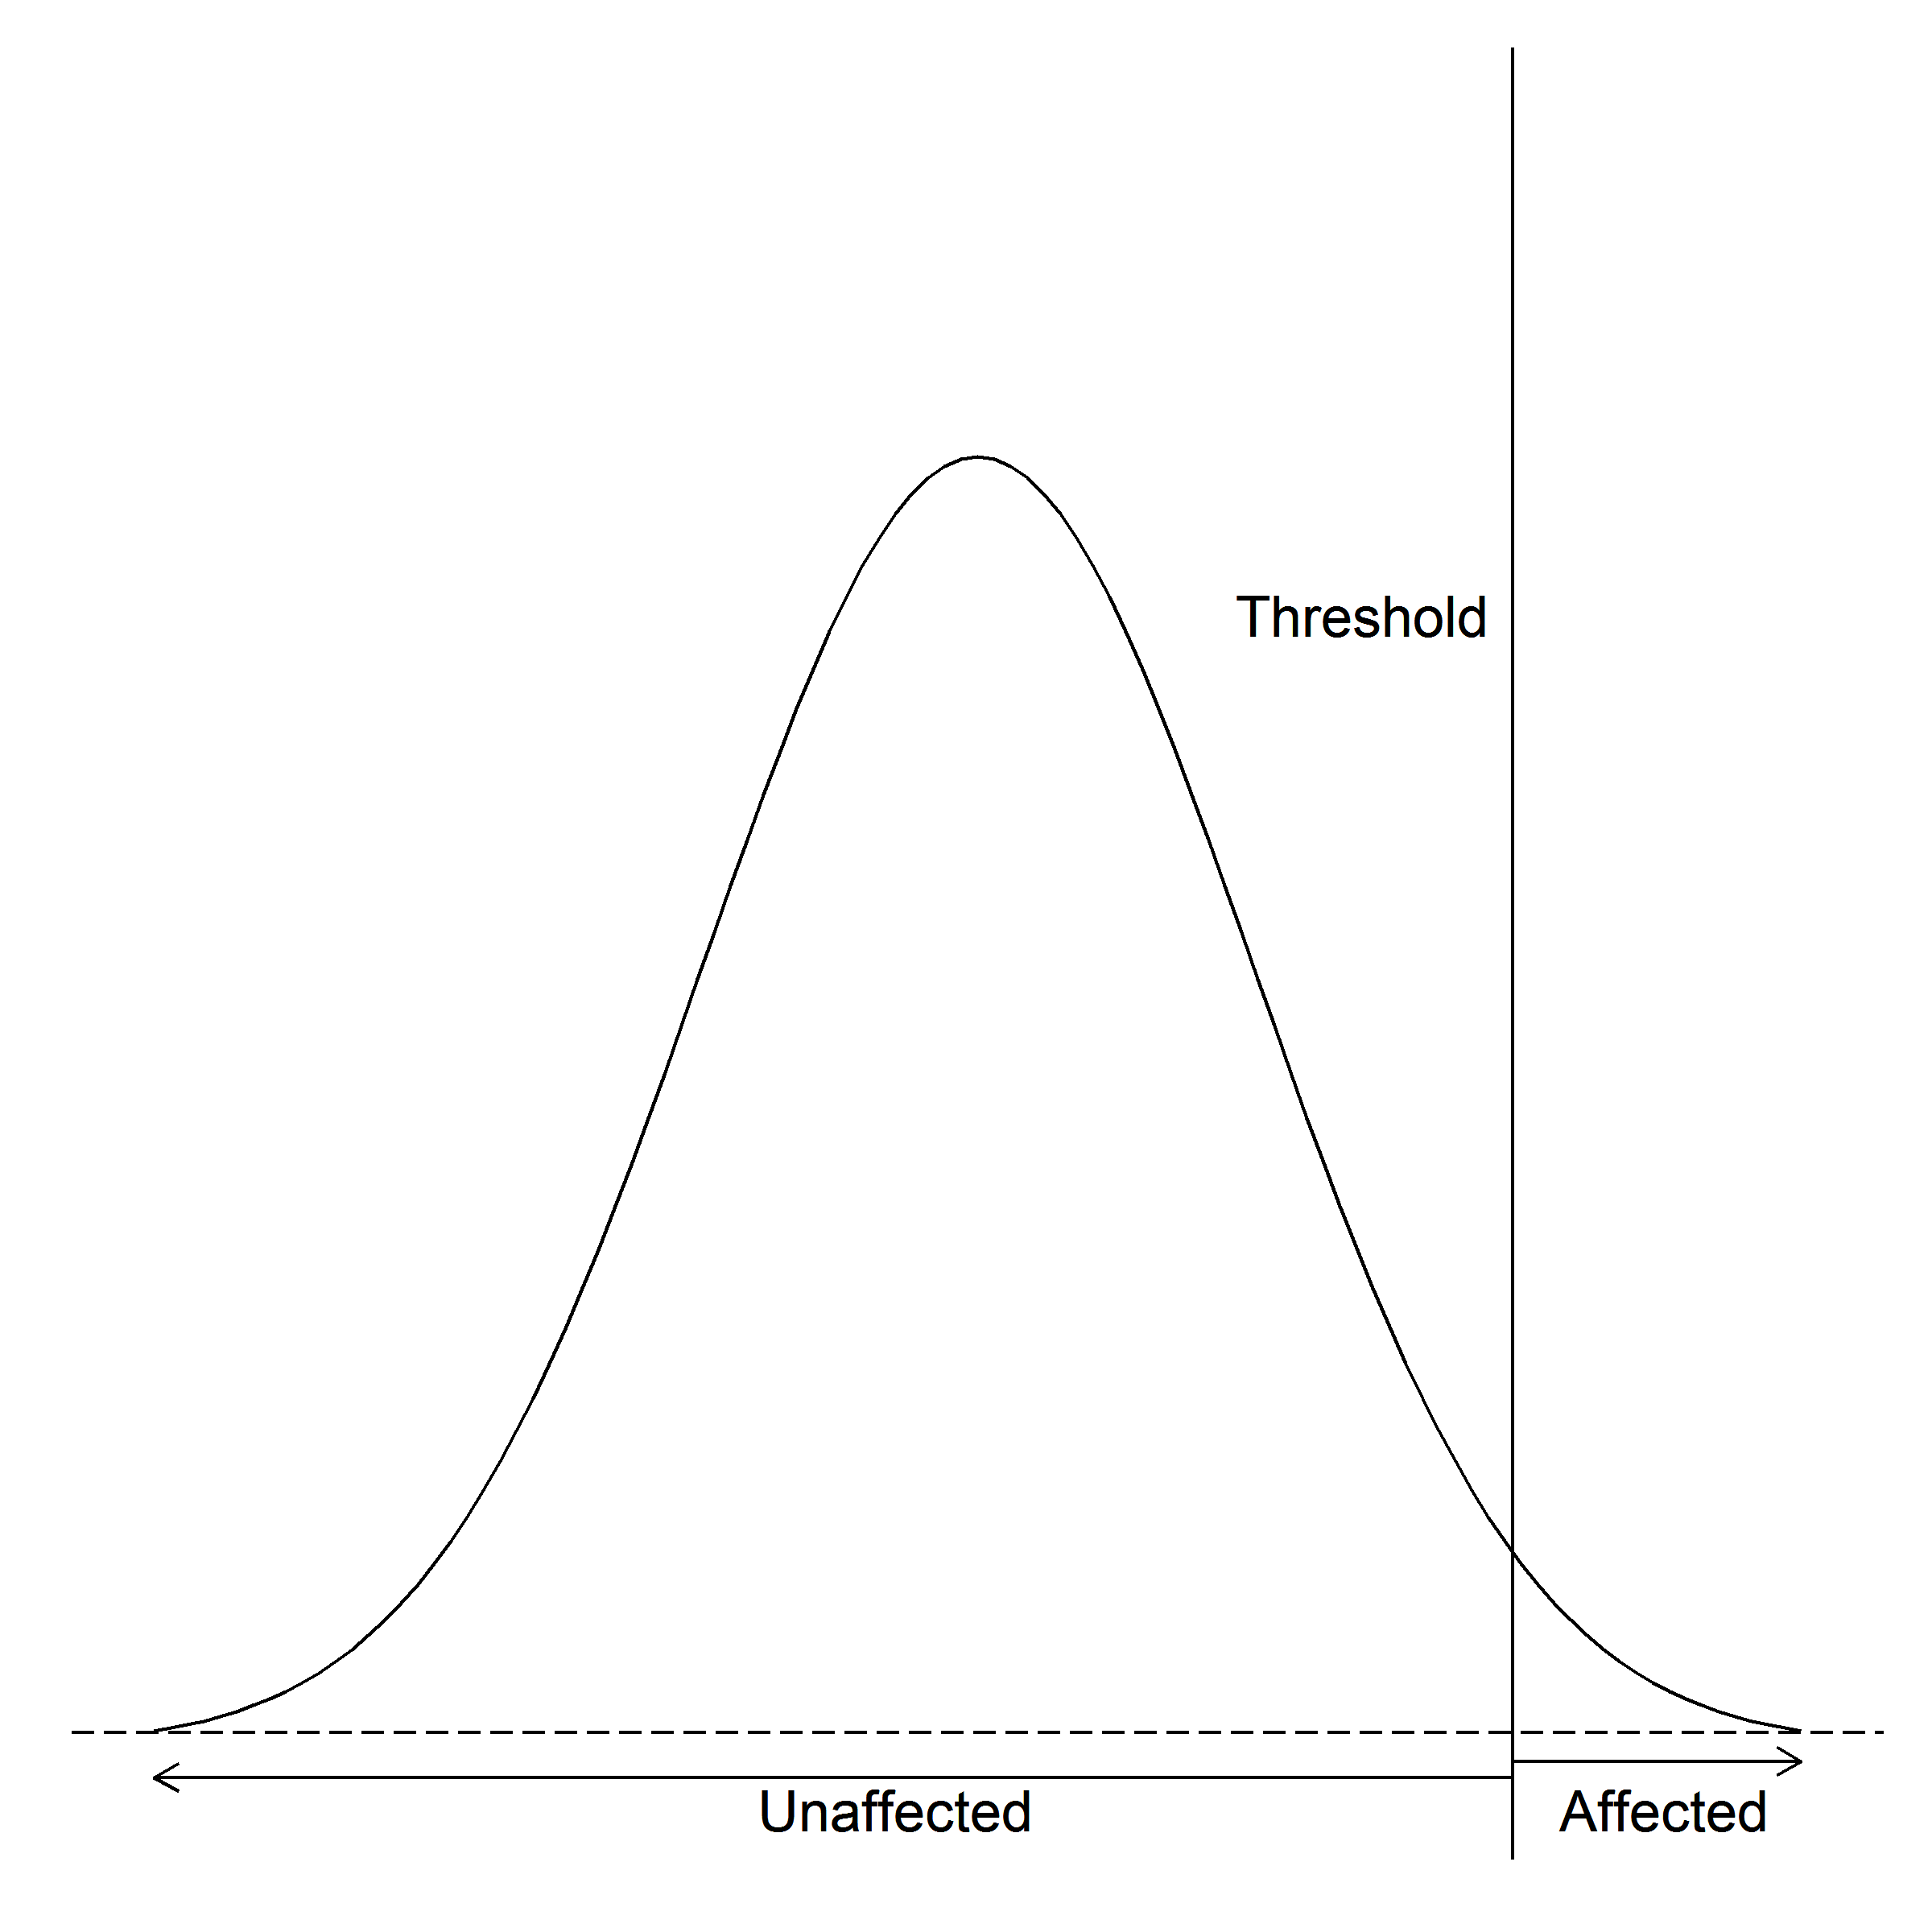
\includegraphics[width=0.5\textwidth]{figure/liability.png}
		\caption[Liability Threshold Model]{
			The liability threshold model.
			Only when an individual has a liability above the liability threshold will he/she be affected.
			}
			\label{fig:liability}
	\end{figure}
	One can then estimate the heritability of the discontinuous by comparing the mean liability of the general population when compared to the relatives of the affected individuals.	
	For example, if we consider a single threshold model of a dichotomous trait, where 
	\begin{align}
	T_G &= \text{Liability threshold of the general population}\notag\\
	T_R &= \text{Liability threshold of relatives of the index case} \notag\\
	q_G &= \text{Prevalence in the general population}\notag\\
	q_R &= \text{Prevalence in relatives of the index case}\notag\\
	L_a &= \text{Mean Liability of the index case} \notag
	\end{align}
	by assuming both the liability distribution of the general population and the relative of the index case both follows the standard normal distribution, we can align the two distribution with respect to $T_G$ and $T_R$. 
	We can then calculate the mean liability of the index case $L_a$ as $L_a=\frac{z_G}{q_G}$ where $z_G$ is the density of the normal distribution at the liability threshold $T_G$.
	Then we can express the regression of relatives' liability on the liability of the index case as
	\begin{align}
	\beta &= \frac{T_G-T_R}{L_a}
	\label{eq:liability}
	\end{align}
	
	Thus, by applying \cref{eq:liability} to \cref{eq:finalNarrow}, we get
	\begin{align}
	h^2 =\frac{T_G-T_R}{rL_a}
	\end{align}
	
	\subsection{Adoption Study}
	% Need to go deeper into twin studies
	The key limitation of \cref{eq:finalNarrow} was its inability to discriminate the genetic factors from the shared environmental factors.
	Such problem arise as family not only shared some of their genes, but they also tends to share some of the environmental factors such as diet. 
	In fact, this was the main reason for researchers to discord the argument that \glng{scz} is a genetic disorder.
	
	A classical adoption study carried out by \citet{HESTON1966} in 1966 set off to discriminate whether if the increased risk of \glng{scz} in relatives of \glng{scz} was caused by the shared environmental factors or the shared genetic factors. 
	An advantages of adoption studies was that if the child was separated from their family early after birth, then the shared environmental factors should be minimized, thus any resemblance between the parent and child should be driven mainly by the shared genetic factors.
	\citet{HESTON1966} collected data of 47 individuals born from a schizophrenic mother during the period from 1915 to 1947. 
	They were separated from their mother within three day of birth and were sent to a foster family. 
	50 matched control were also recruited to the study.
	It was observed that there was an increased risk of \glng{scz} in individual born to schizophrenic mother when compared to the control group even-though they were brought up in a different environment as that of their mother.
	This result suggested that \glng{scz} was likely driven by the shared genetic factors instead of the shared environmental factors.
	
	\subsection{Twin Studies}
	Despite the usefulness of adoption studies in delineating the effect of shared environment from the genetic factors, collection of adoption data were difficult. 
	Moreover, any prenatal influence such as alcohol abuse during pregnancy might confound the results.
	Therefore, an alternative way would be the twin studies using the relationship between the \gls{mz} and \gls{dz} twins.
	
	Theoretically, \gls{mz} twins should share all their genetic components (both additive ($A$) and non-additive ($D$) genetic factors) and also their common environmental factors ($C$) where the only difference between a twin pair would be the non-shared environmental factors ($E$). 
	As for the \gls{dz} twins, they also share the same common environmental factors yet they only share $\frac{1}{2}$ of their additive genetic factors and $\frac{1}{4}$ of their non-additive genetic factors. 
	The non-shared environmental was also by definition not shared among the twins \citep{Rijsdijk2002}.
	Based on these assumptions, \cite{Falconer1996} derived the heritability as
	\begin{equation}
	h^2 = 2(\rho_{MZ}-\rho_{DZ})
	\end{equation}
	where $\rho_{MZ}$ and $\rho_{DZ}$ were the phenotype correlation between the \gls{mz} twins and \gls{dz} twins respectively.
	
	By combining Falconer's formula and the concept of liability threshold model, \citet{Gottesman01071967} estimated that the heritability of \glng{scz} to be $>60\%$ based on previously collected twin data, strongly suggest \glng{scz} as a genetic disorder.
	The result was further supported by one of the landmark meta-analysis study conducted by \citet{Sullivan2003}.
	Based on data obtained from 12 published \glng{scz} twin studies, \citet{Sullivan2003} found that although there was a non-zero contribution of environmental influence on liability of \glng{scz} ($11\%$, \gls{ci}=$3\%-19\%$), there was a much larger contribution from genetics ($81\%$, \gls{ci}=$73\%-90\%$), further supporting that \glng{scz} was largely mediated by the genetic factors.
	
	Such findings were not limited to twin-studies but were also reported in large scale population based studies.
	A recent large scale population based study in Sweden population \citep{Lichtenstein2009} also found that there was a large genetic contribution in \glng{scz} ($64\%$).
	Although the estimated heritability (64\% \citep{Lichtenstein2009} vs 81\% \citep{Sullivan2003}) differs between the two studies, there is no doubt that \glng{scz} is highly heritable, leading to the initiative of genetic research in \glng{scz}.
	
	\section{Schizophrenia Genetics}
	The results from the twin studies strongly support \glng{scz} as a genetic disorder.
	However, little was known about the mechanism of \glng{scz} nor the genetic architecture of the disorder. 
	All data from adoption studies, twin studies and family studies shown that \glng{scz} does not follow the Mendelian framework \citep{Gottesman01071967,Gottesman1982}.
	Specifically, shall \glng{scz} be a Mendelian disorder, then we would expect all \gls{mz} siblings of the proband to also suffer from \glng{scz}.
	However, the life time morbid risk of monozyogitc twins were only $48\%$ (\cref{fig:lifeMRscz}) \citep{gottesman1991schizophrenia}, making it unlikely for \glng{scz} to follow a Mendelian pattern.
	\begin{figure}[t]
		\centering
		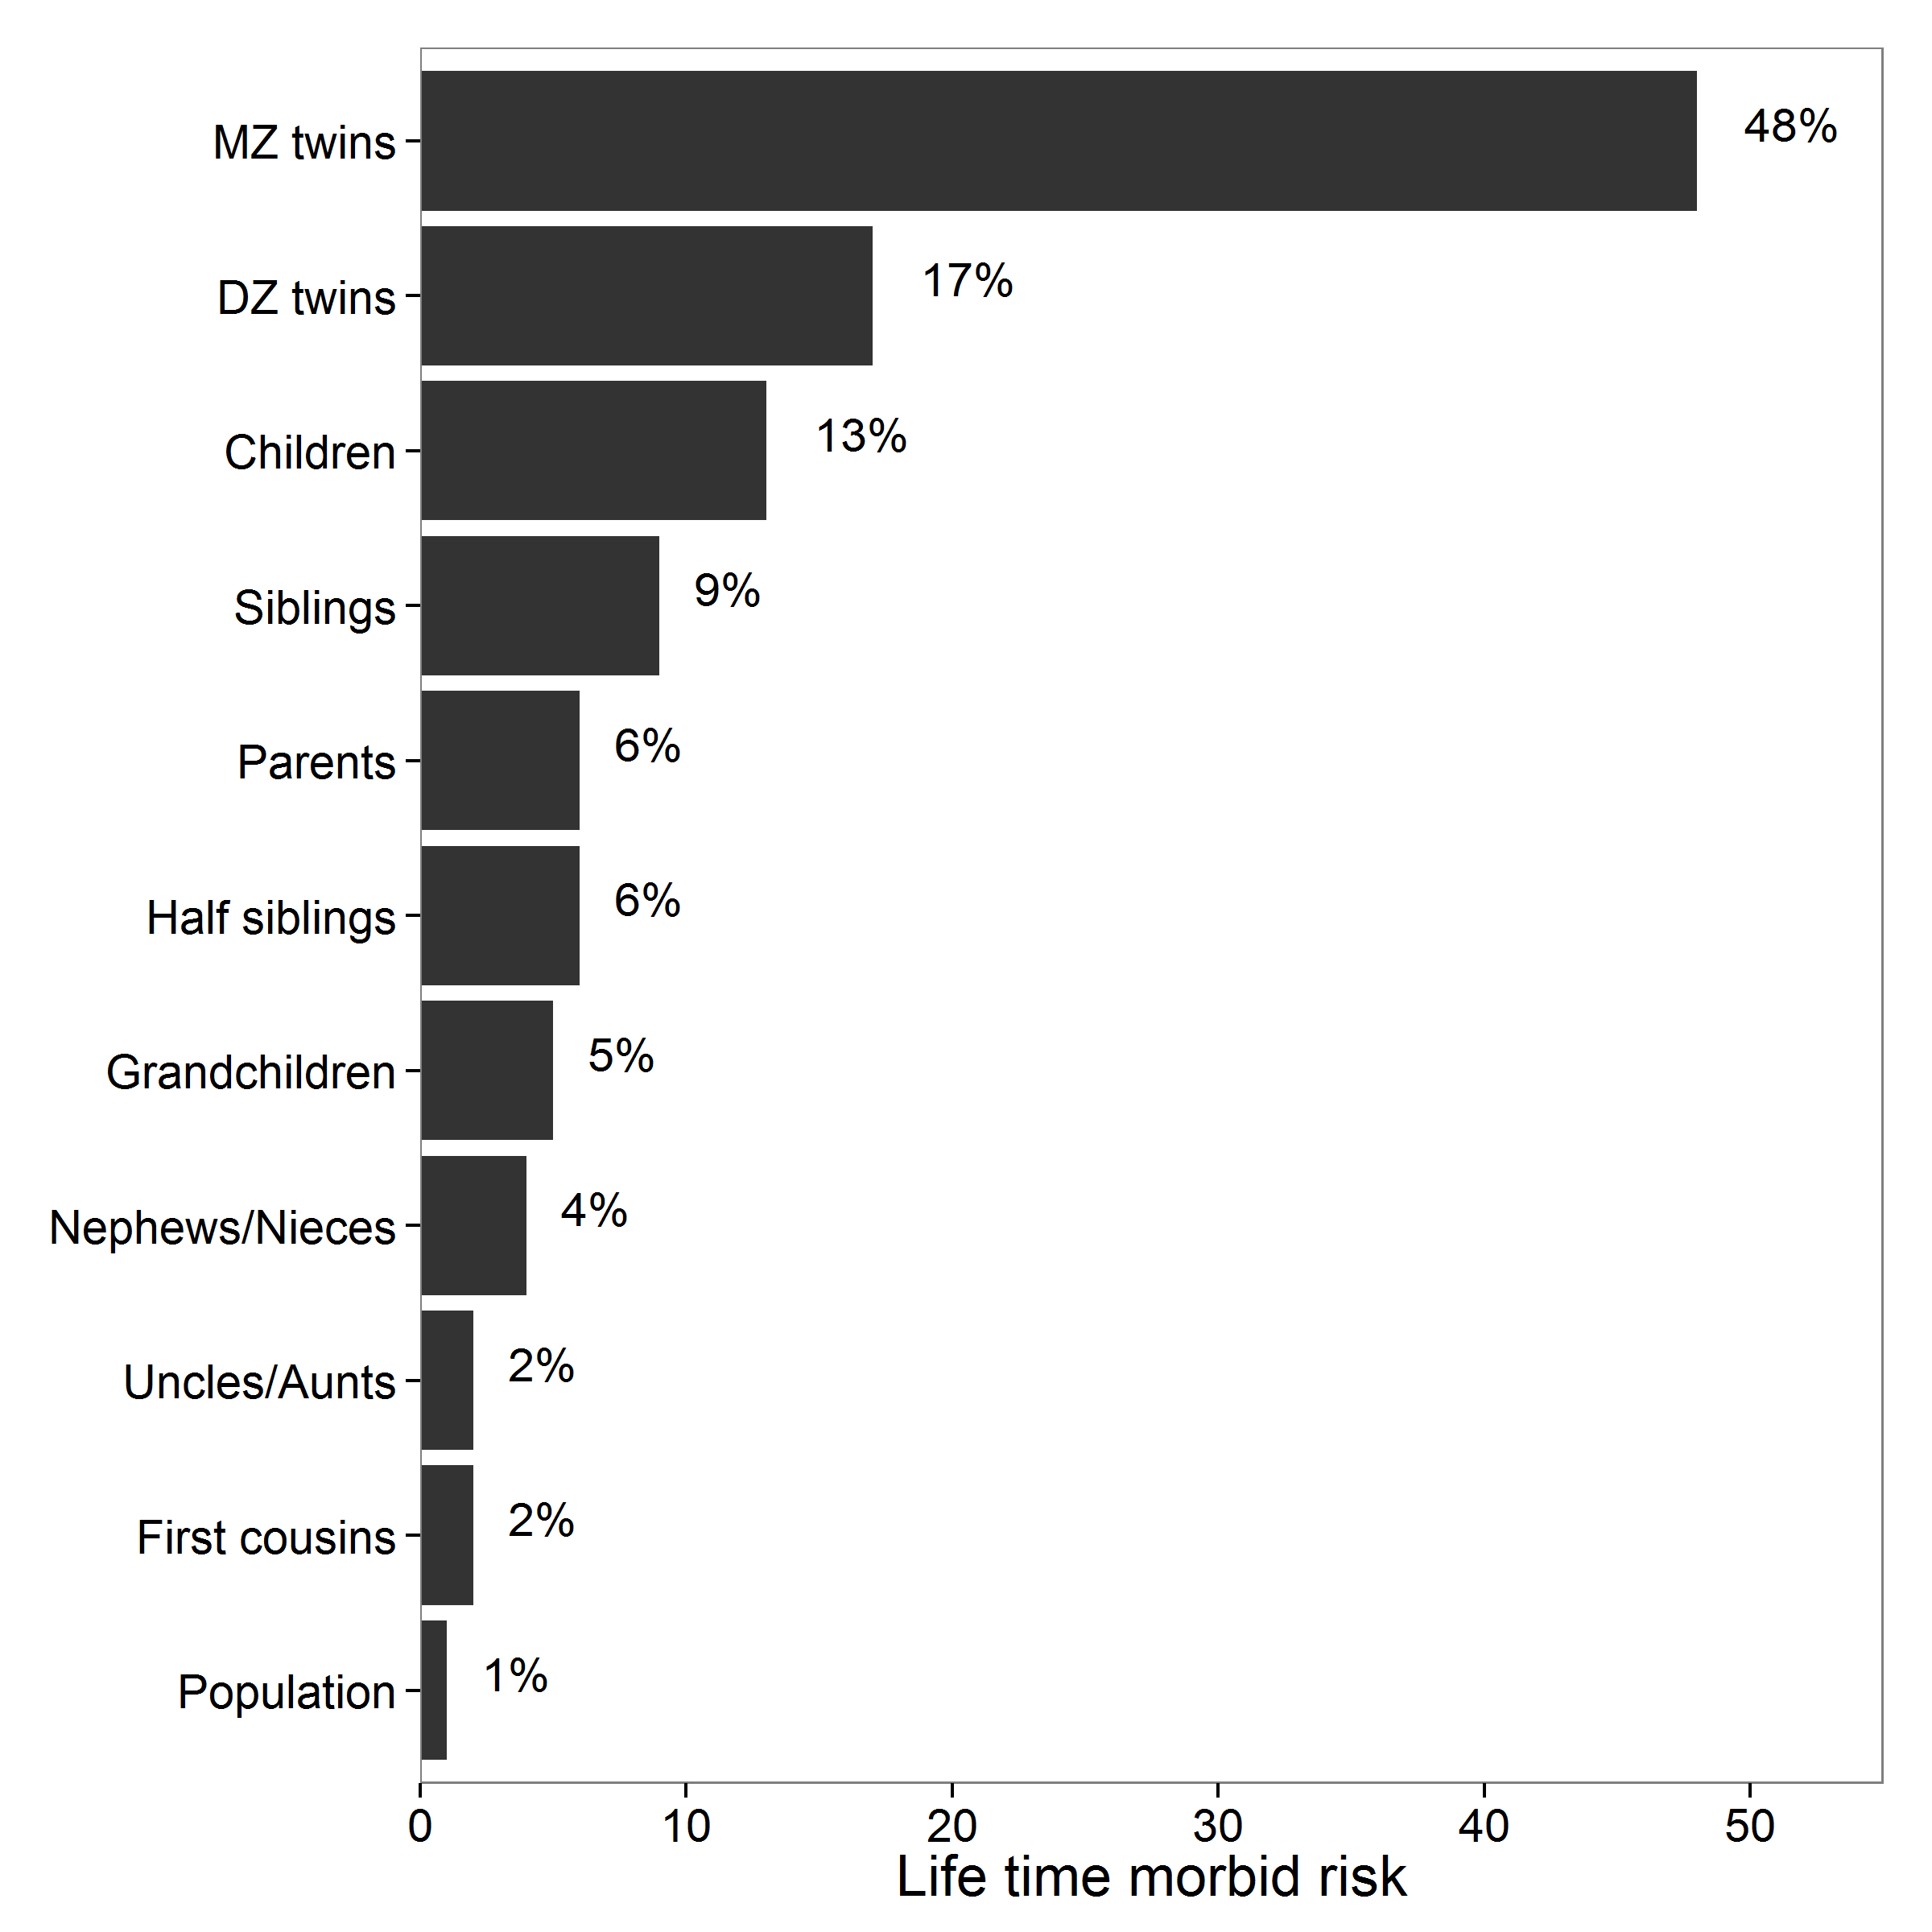
\includegraphics[width=0.6\textwidth]{figure/lifeTimeMorbidRisk.png}
		\caption[Lifetime morbid risks of \glng{scz} in various classes of relatives of a proband]{Lifetime morbid risks of \glng{scz} in various classes of relatives of a proband.
			It was noted that the morbid risk of monozygotic (MZ) twins were only $48\%$, much lower than one would expect if \glng{scz} follows a Mendelian pattern.
			Reproduced with permission from journal \citep{Riley2006}. \label{fig:lifeMRscz}}
	\end{figure}
	
	
	Based on these observations, \citet{Gottesman1967} proposed that \glng{scz} follows a polygenic model where disease phenotype were determined by the additive effects from multiple genes.
	Thus, \glng{scz} is likely to be a complex genetic disorder with complicated pattern of inheritance. 
	Their hypothesis was supported by the calculation of \citet{Risch1990a}.
	
	Not only does \citet{Risch1990a} supports the polygenic model for schizophrenia, \citet{Risch1990a} also estimated the possible effect size of individual locus in schizophrenia. 
	By comparing the observed life time morbid risk and the expected risk from different models, \citet{Risch1990a} proposed that genetic models with a single locus with risk of 3.0 and with all other loci of small effect or models with two or three loci with risk of 2.0 were most consistent with the observed life time morbid risk of \glng{scz} \citep{Risch1990}.
	
	\citet{Risch1990a}'s calculation provided an explanation for the early inconsistent findings of linkage studies in \glng{scz} \citep{Harrison2005}.
	As linkage studies were aimed to identify genetic variation of large effect size they failed to capture genetic loci with small effect size.
	It was therefore tempting to suggest that \glng{scz} only follows the ``common disease-common variant'' model, which stated that \glng{scz} is mediated by large amount of common variants such as \glng{SNP}, each carries a small effect size.
	
	However, another possible hypothesis was that the variation mediating \glng{scz} were rare, therefore require a large sample size to detect and the inconsistent results of early linkage studies might be due to the inadequate sample size. 
	This lead to some researchers suggesting the ``common disease-rare variant'' hypothesis, which propose that \glng{scz} was mediated by a small amount of rare variants, each with a large effect size \citep{McClellan2007}.
	
	Nevertheless, success in genetic research of \glng{scz} remains limited.
	Only until the initiation of Human Genome Project and technological advance resulted from that does genetic research of \glng{scz} entered an era of success.
	
	\subsection{The Human Genome Project and HapMap Project}
	\glsreset{SNP}
	\glsreset{LD}
	In 1990, the Human genome project was initiated, aiming at constructing the first physical map of the human genome at per nucleotide resolution \citep{Lander2001}.
	The completion of the human genome project has opened up a new era of genetic research, allowing researchers to identify \glspl{SNP} on the human genome, which is one of the major source of genetic variation.
	
	Soon after the completion of the human genome project, the HapMap Project was initiated \citep{Consortium2005}, aiming to provide a genome-wide database of common human sequence variation such as \glspl{SNP} with \gls{maf} $\ge0.05$.
	More importantly was that the HapMap Project also provided a detailed \gls{LD} map of the human genome.
	
	\gls{LD} was of particular importance to genetic research for it was the non-random correlation of genotypes between 2 genetic loci. 
	\glspl{SNP} in high \gls{LD} were usually observed together in the human genome.
	When a large amount of \glspl{SNP} were in high \gls{LD} together, they form what was known as a \gls{LD} block.
	By performing association testing on \glspl{SNP} representing a \gls{LD} block (``tagging''), one can avoid the need of performing association on the whole genome, therefore reducing the cost of the experiment.
	This was the fundamental concept of \gls{GWAS} which was now extensively used in the genetic research.
	
	\subsection{Genome Wide Association Study}
	In \gls{GWAS}, genome-wide genotyping array were commonly used to systematically detect common genetic variants such as \gls{SNP} and \gls{cnv}.
	For quantitative traits, the association between the trait and frequency of the variants were calculated using methods such as linear regression.
	On the other hand, for dichotomous traits such as \glng{scz}, the frequency of the variants were compared between the case and control samples using methods such as chi-square test or logistic regression.
	Because of the problem of multiple testing, only variants with a p-value passing a genome wide threshold (p-value $\le5\times10^{-8}$) were considered significant.
	Another possible method to decide the significant threshold was to consider the ``effective number'' of tests \citep{Li2011}, which reduced the genome wide threshold according to the \gls{LD} structure.
	When designing a \gls{GWAS}, one need to take into account of the magnitude of effect, sample size, and required level of statistical significance (the false-positive, or type I, error rate) in order to have a powerful study \citep{Purcell2003}.
	
	\subsubsection{The Success of Psychiatric Genomic Consortium} 
	Despite the great promise from \gls{GWAS}, early \gls{GWAS} in \glng{scz} remain largely disappointing and were unable to identify any robust genetic markers associated with \glng{scz}.
	The failure of early \gls{GWAS} in \glng{scz} were mainly due to the relative small sample size of the studies, which result in low detection power.
	
	To overcome the problem of small sample size, large consortium were formed such that data from different research groups from different countries were combined, which provides a large sample size for the analysis.
	By 2014, the \Glng{scz} Working group of the \gls{pgc} has collected a total of 36,989 \glng{scz} samples and 113,075 controls for the meta-analysis of \glng{scz} \citep{Ripke2014}.
	In their study \citep{Ripke2014}, 128 linkage-disequilibrium-independent \glspl{SNP} were found to  exceeded the genome-wide significance (p-value $\le 5\times10^{-8}$), corresponding to 108 genetic loci.
	75\% of these loci contain protein coding genes and a further 8\% of these loci were within 20\gls{kb} of a gene. 
	It was found that genes involved in glutamatergic neurotransmission (e.g. \textit{GRM3}, \textit{GRIN2A} and \textit{GRIA1}), synaptic plasticity and genes encoding the voltage-gated calcium channel subunits (e.g. \textit{CACNA1C}, \textit{CACNB2} and \textit{CACNA1I}) were among the genes associated within these loci.
	Importantly, \textit{DRD2}, the target of all effective anti-psychotic drug were also associated with \glng{scz}.
	This result converges with existing knowledge of \textit{DRD2} being involved in the pathology of \glng{scz}, supported by multiple lines of research \citep{Talkowski2007}.
	\begin{figure}
		\centering
		\caption[Enrichment of enhancers of SNPs associated with Schizophrenia]{Enrichment of enhancers of SNPs associated with \glng{scz}. 
			It was observed that the largest enrichment were in cell lines related to the brain and in tissues with important immune functions. 
			Graphs reproduced with permission from the journal \citep{Ripke2014}.}
		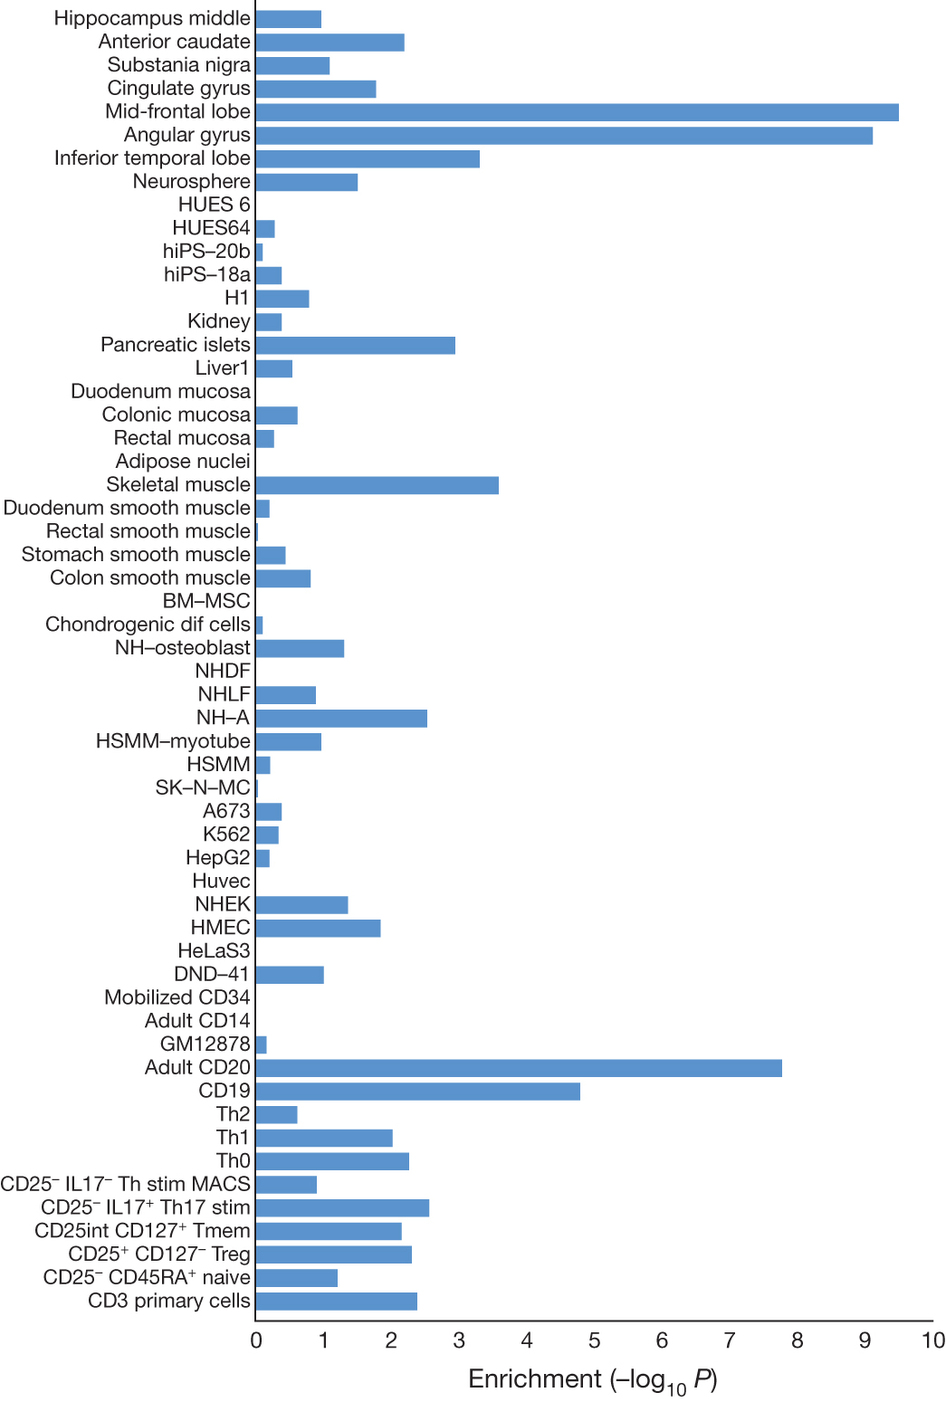
\includegraphics[height=\textwidth]{figure/pgc_enrichment_tissue.jpg}
		\label{fig:pgcEnrich}
	\end{figure}
	It was further demonstrated that \glng{scz} association were significantly enriched at enhancers active in brain and enriched at enhancers active in tissues with important immune functions (\cref{fig:pgcEnrich})\citep{Ripke2014}.
	
	The enrichment of immune related enhancers remains significant even after the removal of \gls{mhc} region from the analysis, provided further genetic support of the involvement of the immune system in the etiology of \glng{scz}.
	Because of its role in neural development \citep{Zhao1998,Deverman2009}, it is likely that the perturbation in the immune system might disrupt the brain development, therefore increasing the risk of \glng{scz}.
	%Indeed, studies on \gls{mia} has demonstrated that cytokine imbalance might predispose individual to \glng{scz} \citep{Meyer2009}. 
	
	Although the \gls{pgc} \glng{scz} \gls{GWAS} is very successful, it is uncertain whether if all common variants associated with \glng{scz} has been captured. 
	With the unknown number of causal loci with moderate-to-small effect size, many \glspl{SNP} associated with \glng{scz} may be left undetected given the current sample size. 
	However, it is also possible that the \gls{pgc} \glng{scz} \gls{GWAS} has already captured all or near most of the \glspl{SNP} associated with the disease. 
	Therefore, estimating the contribution of these common \glspl{SNP} to \glng{scz} has important implications for future research strategy.
	
	\subsection{Contribution of Common SNPs}
	In a typical \gls{GWAS}, a stringent genome wide significant threshold were usually employed to avoid false positive findings. 
	However, if individual \glspl{SNP} have a small effect on the trait, the real association might be missed.
	Therefore, to estimate the true contribution of common \glspl{SNP} to a disease (\gls{SNP}-heritability), one should try to use all \glspl{SNP} in the estimation.
	
	\subsubsection{Genome-wide Complex Trait Analysis}
	Currently, the most popular algorithm used for the estimation of \gls{SNP}-heritability is \gls{gcta}, which uses information from the \gls{grm} \citep{Yang2011}.
	The \gls{grm} is represents the ``genetic distance'' between all individuals within the \gls{GWAS}.
	Genetic relationship between individual $j$ and $k$ is estimated as 
	\begin{equation}
	A_{jk} = \frac{1}{N}\sum^N_{i=1}\frac{(x_{ij}-2p_i)(x_{ik}-2p_i)}{2p_i(1-p_i)}
	\end{equation}
	where $x_{ij}$ is the number of copies of the reference allele for the $i^{th}$ \gls{SNP} of the $j^{th}$ individual and $p_i$ is the frequency of the reference allele.
	This is based on the fact that genotypes were usually coded as 0, 1 or 2 (homozygous reference, heterozygous and homozygous alternative respectively) and should follow the binomial distribution.
	From the binomial distribution, the expected mean and variance of the genotype $i$ will be $2p_i$ and $2p_i(1-p_i)$ respectively.
	Thus $A_{jk} = \frac{1}{N}\sum^N_{i=1}z_{ij}z_{ik}$ where $z_{ij}$ is the standardized genotype for the $i^{th}$ \gls{SNP} of the $j^{th}$ individual.
	
	Using the information from the \gls{grm}, \citet{Yang2011} then fit the effects of all the \glspl{SNP} as random effects by a \gls{mlm}
	\begin{align}
	\boldsymbol{y} &= \boldsymbol{X\beta}+\boldsymbol{g}+\epsilon\\
	\mathrm{Var}(\boldsymbol{y}) &= \boldsymbol{A}\sigma_g^2+\boldsymbol{I}\sigma_\epsilon^2
	\end{align}
	where $\boldsymbol{y}$ is an $n\times 1$ vector of phenotypes with $n$ samples, $\boldsymbol{\beta}$ is a vector of fixed effects such as sex and age, $\boldsymbol{g}$ is an $n\times 1$ vector of the total genetic effects of the individuals, $\sigma_g^2$ is the variance explained by all the \glspl{SNP} and finally, $\sigma_\epsilon^2$ is the variance explained by residual effects.

	The main concept of \gls{gcta} is that instead of testing the associations for individual \glspl{SNP}, one fit the effects of all \glspl{SNP} as random effects in a \gls{mlm} and estimate a single parameter, i.e. the variance explained by all \glspl{SNP} or \gls{SNP}-heritability.
	Given the information of the \gls{grm}, \citet{Yang2011} implemented the \gls{reml} using the average information algorithm to estimates the $\sigma_g^2$ and $\sigma_\epsilon^2$where the \gls{reml} is a form of maximum likelihood estimation that allows unbiased estimates of variance and covariance parameters.
	The \gls{SNP}-heritability of the trait is then defined as $\frac{\sigma_g^2}{\sigma_g^2+\sigma_e^2}$.

	Based on the above concept, \citet{Yang2010a} were able to estimate the variance in height explained by \glspl{SNP} from the height \gls{GWAS} to be around 45\%, much larger than previously reported 5\%.
	The main difference in the estimates was because the \gls{mlm} \gls{reml} were able to consider all \glspl{SNP} simultaneously without limited on significant \glspl{SNP}.
	Although the estimates was still less than 80\% which was the expected heritability of height, \citet{Yang2010a} was able to demonstrated that one possible source of ``missing heritability'' might be due to incomplete \gls{LD}.
	By taking into consideration of incomplete \gls{LD}, it was estimated that the proportion of variance explained by causal variants can be as high as 0.84 with \gls{se} of 0.16 \citep{Yang2010a}, close to the expected heritability.
	Together, \citet{Yang2011} provide a possible method for the estimation of the variance explained by \glspl{SNP} in \gls{GWAS} data and the method is now implemented in \gls{gcta} which is wildly adopted.
	
	The problem with \gls{gcta} was that genotype data are required to calculate the \gls{grm}.
	For complex disease like \glng{scz}, the data were usually obtained from multiple data source where the raw genotypes were unavailable due to privacy concerns.
	Instead, summary statistics were usually provided.
	Therefore estimation of variance explained by \glspl{SNP} in these \gls{GWAS} can only rely on the summary statistics. 
	
	\subsubsection{\glng{ldsc}}
	In large scale \gls{GWAS} studies, a general inflation of summary statistics can sometimes be observed.
	It was usually considered to be contributed by the presence of confounding factors such as population stratification, under the assumption that most of the \glspl{SNP} should have no association to the disease.
	It was therefore a common practice for one to perform the \gls{gc} on the \gls{GWAS} results \citep{Zheng2006}.
	
	The problem of \gls{gc} was that the basic assumption of a small number of causal \glspl{SNP} might not be true, especially in complex disease like \glng{scz}.
	Through careful simulation, \citet{Yang2011b} demonstrated that in the absence of population stratification and other form of technical artifacts, the presence of polygenic inheritance can inflate the summary statistic \citep{Yang2011b}.
	More importantly, they observed that the magnitude of inflation was determined by the \emph{heritability}, the \gls{LD} structure, sample size and the number of causal \glspl{SNP} of the trait.
	
	The observation of \citet{Yang2011b} provide important foundation for the estimation of \gls{SNP} heritability based on summary statistics where a possible method will be to elucidate the heritability based on the magnitude of inflation of the summary statistics. 
	However, when confounding factors such as population stratification and cryptic relatedness are presented, they can also inflate the summary statistics.
	Therefore, in order to estimate the \gls{SNP}-heritability, one must be able to delineate the confounding factors from the polygenicity of the trait.
	
	Based on the work of \citet{Yang2011b}, \citet{Bulik-Sullivan2015} hypothesized that strength of ``tagging'' of a \gls{SNP} should be correlated with the probability of it to ``tag'' the causal \gls{SNP} yet should be independent to confounding factors such as population stratification and cryptic relatedness.
	\citet{Bulik-Sullivan2015} then define the strength of ``tagging'' of a \gls{SNP} as the \gls{LD} score, which is the sum of $r^2$ of $k$ \glspl{SNP} within a 1cM window of \gls{SNP}$_j$:
	\begin{equation}
	l_j = \sum_kr^2_{jk}
	\label{eq:ldScore}
	\end{equation}
	
	Based on their hypothesis, the expected $\chi^2$ of association of \gls{SNP}$_j$ with the trait can be defined as a function of the \gls{LD} score ($l_j$), the number of samples ($N$), the number of \glspl{SNP} in the analysis($M$) and most importantly, the \gls{SNP} heritability ($h^2$):
	\begin{equation}
	\mathrm{E}[\chi^2_j | l_j] = \frac{Nh^2}{M}l_j+1
	\label{eq:fixedLDSC}
	\end{equation}
	%TODO understand the exact calculation of LDSC
	
	When confounding factors were present in the study (e.g. population stratification), \cref{eq:fixedLDSC} can instead be defined as
	\begin{equation}
	\mathrm{E}[\chi^2_j | l_j] = \frac{Nh^2}{M}l_j+Na+1
	\label{eq:fullLDSC}
	\end{equation}
	where $a$ is the contribution of confounding bias.
	
	By considering \cref{eq:fullLDSC} as a regression model, \citet{Bulik-Sullivan2015} observed that the contribution of common variants (the \gls{SNP} heritability $h^2$) will be the slope of the regression and the intercept minus one will represent the mean contribution of the confounding bias such as those of population stratification. 
	The \gls{ldsc} was implemented by \citet{Bulik-Sullivan2015}, hoping to use \cref{eq:fullLDSC} to delineate the contribution from confounding factors and common genetic variants.
	
	To test their hypothesis, \citet{Bulik-Sullivan2015} simulated multiple \gls{GWAS} where the trait can have a polygenic architecture or where confounding factors can present.
	When the simulated trait is polygenic and no confounding factors were presented, the average \gls{ldsc} intercept was close to one and the estimates were unbiased in all situation.
	Only when the number of causal variants was small will the standard error of the estimates become very large.
	On the other hand, when the \gls{GWAS} was simulated with only the confounding factors such as population stratification, the intercept estimated was approximately equal to the \gls{gc} inflation factor with only a small positive bias in the regression slope.
	
	Moreover, when a polygenic trait was simulated with confounding factors, the intercept of \gls{ldsc} was approximately equal to the mean $\chi^2$ statistic among the null \glspl{SNP}, providing strong evidence that \gls{ldsc} can partition the inflation in test statistic even in the presence of both bias and polygenicity.
	
	Given  the success of the simulation, \citet{Bulik-Sullivan2015} estimated the \gls{SNP} heritability of \glng{scz} using the summary statistics from the \gls{pgc} \glng{scz} \gls{GWAS} \citep{Ripke2014}.
	By applying the liability threshold adjustment, \citet{Bulik-Sullivan2015} estimated the \gls{SNP}-heritability of \glng{scz} should be 0.555 with \gls{se} of 0.008.
	The estimated \gls{SNP} heritability was lower than the heritability estimated from population based study (64\% \citep{Lichtenstein2009}) and twin studies (81\% \citep{Sullivan2003}) suggesting that it is possible for variants other than common \glspl{SNP} to account for variations in \glng{scz}.
	
	\subsubsection{Partitioning of Heritability}
	Another implication of \gls{ldsc} is that it allows the partitioning of heritability, which allow one to identify pathways that were associated with a trait.
	
	Traditionally, functional enrichment analysis in \gls{GWAS} only take into account of \glspl{SNP} that passed the genome wide significance threshold. 
	However, for complex traits such as that of \glng{scz}, much of the heritability might lies in \glspl{SNP} that do not reach genome wide significance threshold at the current sample size.
	For example, in 2013, only 13 risk loci were detected using 13,833 \glng{scz} samples and 18,310 controls \citep{Ripke2013}. 
	When the sample size increased to 34,241 \glng{scz} samples and 45,604 controls in 2014, 108 risk loci were identified \citep{Ripke2014}. 
	Thus, if one only consider the significant loci, risk loci that have not reach genome wide significance threshold might be ignored from the analysis, decreasing the power of the functional enrichment analysis.

	In order to estimate whether if a functional categories was associated with the trait, \gls{ldsc} takes into consideration of the summary statistic of all the \glspl{SNP}.
	The partitioning of the heritability is then calculated as 
	\begin{equation}
	\mathrm{E}[\chi^2_j] = N\sum_C\tau_Cl(j,C)+Na+1
	\label{eq:partitionH}
	\end{equation}
	
	The main difference between \cref{eq:partitionH} and \cref{eq:fullLDSC} is that $\frac{h^2}{M}l_j$ is substituted by $\sum_C\tau_Cl(j,C)$ where $l(j,C)$ is the \gls{LD} Score of \gls{SNP} $j$ with respect
	to category $C$ and $\tau C$ is the per-\gls{SNP} heritability in category $C$.
	
	Using data from \citet{Ripke2014} and functional categories derived from the ENCODE annotation \citep{ENCODEProjectConsortium2012}, the NIH Roadmap Epigenomics Mapping Consortium annotation \citep{Bernstein2010} and other studies, \citep{Finucane2015} tried to identify functional categories that were most enriched in \glng{scz}.
	In their study, it was found that brain cell types were most enriched in \glng{scz}, especially those related to the \gls{cns}.
	Of all the functional categories, the most enriched category in \glng{scz} was the H3K4me3 mark in the fetal brain(\cref{tab:cellTypeScz}). 
	As H3K4me3 was mostly linked to active promoters, this suggest that genes that were activated in fetal brain (e.g. genes related to brain development) were associated with \glng{scz}, supporting the idea of \glng{scz} as a neuro-developmental disorder. 
		
	Moreover, it was also observed that the second most enriched cell types were those related to immunity.
	Undoubtedly, the \gls{cns} and the immune system have an important role in the disease etiology of \glng{scz}. 
		
	\begin{singlespace}
		\begin{longtable}{p{6cm}rrr}
			%\begin{tabular}{rrrr}
			\toprule
			Cell type & cell-type group & Mark  & P-value \\
			\midrule
			Fetal brain** & CNS   & H3K4me3 & $3.09\times 10^{-19}$ \\
			Mid frontal lobe** & CNS   & H3K4me3 & $3.63\times 10^{-15}$ \\
			Germinal matrix** & CNS   & H3K4me3 & $2.09\times 10^{-13}$ \\
			Mid frontal lobe** & CNS   & H3K9ac & $5.37\times 10^{-12}$ \\
			Angular gyrus** & CNS   & H3K4me3 & $1.29\times 10^{-11}$ \\
			Inferior temporal lobe** & CNS   & H3K4me3 & $1.70\times 10^{-11}$ \\
			Cingulate gyrus** & CNS   & H3K9ac & $5.37\times 10^{-11}$ \\
			Fetal brain** & CNS   & H3K9ac & $5.75\times 10^{-11}$ \\
			Anterior caudate** & CNS   & H3K4me3 & $2.19\times 10^{-10}$ \\
			Cingulate gyrus** & CNS   & H3K4me3 & $4.57\times 10^{-10}$ \\
			Pancreatic islets** & Adrenal/Pancreas & H3K4me3 & $2.24\times 10^{-09}$ \\
			Anterior caudate** & CNS   & H3K9ac & $3.16\times 10^{-9}$ \\
			Angular gyrus** & CNS   & H3K9ac & $4.68\times 10^{-9}$ \\
			Mid frontal lobe** & CNS   & H3K27ac & $7.94\times 10^{-9}$ \\
			Anterior caudate** & CNS   & H3K4me1 & $1.20\times 10^{-8}$ \\
			Inferior temporal lobe** & CNS   & H3K4me1 & $3.72\times 10^{-8}$ \\
			Psoas muscle** & Skeletal Muscle & H3K4me3 & $4.17\times 10^{-8}$ \\
			Fetal brain** & CNS   & H3K4me1 & $6.17\times 10^{-8}$ \\
			Inferior temporal lobe** & CNS   & H3K9ac & $9.33\times 10^{-8}$ \\
			Hippocampus middle** & CNS   & H3K9ac & $9.33\times 10^{-7}$ \\
			Pancreatic islets** & Adrenal/Pancreas & H3K9ac & $1.62\times 10^{-6}$ \\
			Penis foreskin melanocyte primary** & Other & H3K4me3 & $2.09\times 10^{-6}$ \\
			Angular gyrus** & CNS   & H3K27ac & $2.34\times 10^{-6}$ \\
			Cingulate gyrus** & CNS   & H3K4me1 & $2.82\times 10^{-6}$ \\
			Hippocampus middle** & CNS   & H3K4me3 & $2.82\times 10^{-6}$ \\
			CD34 primary** & Immune & H3K4me3 & $4.68\times 10^{-6}$ \\
			Sigmoid colon** & GI    & H3K4me3 & $5.01\times 10^{-6}$ \\
			Fetal adrenal** & Adrenal/Pancreas & H3K4me3 & $6.31\times 10^{-6}$ \\
			Inferior temporal lobe** & CNS   & H3K27ac & $8.32\times 10^{-6}$ \\
			Peripheralblood mononuclear primary** & Immune & H3K4me3 & $9.33\times 10^{-6}$ \\
			Gastric** & GI    & H3K4me3 & $1.17\times 10^{-5}$ \\
			Substantia nigra* & CNS   & H3K4me3 & $1.95\times 10^{-5}$ \\
			Fetal brain* & CNS   & H3K4me3 & $2.63\times 10^{-5}$ \\
			Hippocampus middle* & CNS   & H3K4me1 & $3.31\times 10^{-5}$ \\
			Ovary* & Other & H3K4me3 & $6.46\times 10^{-5}$ \\
			CD19 primary (UW)* & Immune & H3K4me3 & $7.08\times 10^{-5}$ \\
			Small intestine* & GI    & H3K4me3 & $8.51\times 10^{-5}$ \\
			Lung* & Cardiovascular & H3K4me3 & $1.17\times 10^{-4}$ \\
			Fetal stomach* & GI    & H3K4me3 & $1.29\times 10^{-4}$ \\
			Fetal leg muscle* & Skeletal Muscle & H3K4me3 & $1.51\times 10^{-4}$ \\
			Spleen* & Immune & H3K4me3 & $1.70\times 10^{-4}$ \\
			Breast fibroblast primary* & Connective/Bone & H3K4me3 & $2.04\times 10^{-4}$ \\
			Right ventricle* & Cardiovascular & H3K4me3 & $2.14\times 10^{-4}$ \\
			CD4+ CD25- Th primary* & Immune & H3K4me3 & $2.19\times 10^{-4}$ \\
			CD4+ CD25- IL17- PMA Ionomycin stim MACS Th sprimary* & Immune & H3K4me1 & $2.19\times 10^{-4}$ \\
			CD8 naive primary (UCSF-UBC)* & Immune & H3K4me3 & $2.24\times 10^{-4}$ \\
			Pancreas* & Adrenal/Pancreas & H3K4me3 & $2.34\times 10^{-4}$ \\
			CD4+ CD25- Th primary* & Immune & H3K4me1 & $2.75\times 10^{-4}$ \\
			CD4+ CD25- CD45RA+ naive primary* & Immune & H3K4me1 & $2.75\times 10^{-4}$\\
			Colonic mucosa* & GI    & H3K4me3 & $3.24\times 10^{-4}$ \\
			Right atrium* & Cardiovascular & H3K4me3 & $3.31\times 10^{-4}$ \\
			Fetal trunk muscle* & Skeletal Muscle & H3K4me3 & $3.39\times 10^{-4}$ \\
			CD4+ CD25int CD127+ Tmem primary* & Immune & H3K4me3 & $3.47\times 10^{-4}$ \\
			Substantia nigra* & CNS   & H3K9ac & $3.63\times 10^{-4}$ \\
			Placenta amnion* & Other & H3K4me3 & $4.17\times 10^{-4}$ \\
			Breast myoepithelial* & Other & H3K9ac & $5.50\times 10^{-4}$ \\
			CD8 naive primary (BI)* & Immune & H3K4me1 & $5.75\times 10^{-4}$ \\
			Substantia nigra* & CNS   & H3K4me1 & $6.61\times 10^{-4}$ \\
			Cingulate gyrus* & CNS   & H3K27ac & $7.94\times 10^{-4}$ \\
			CD4+ CD25- CD45RA+ naive primary* & Immune & H3K4me3 & $8.71\times 10^{-4}$ \\
			\bottomrule
				%\end{tabular}%
			\caption[Enrichment of Top Cell Type of Schizophrenia]{Enrichment of Top Cell type of Schizophrenia.
				* = significant at False Discovery Rate $<$ 0.05.
				** = significant at p $<$ 0.05 after correcting for multiple hypothesis. 
				Reproduce with permission from Journal.\citep{Finucane2015}}
			\label{tab:cellTypeScz}%
		\end{longtable}%
	\end{singlespace}
		
	\subsection{Rare Variants in Schizophrenia}
	\glsreset{cnv}
	The estimated \gls{SNP}-heritability using the common variants captured by the \gls{pgc} \glng{scz} \gls{GWAS} suggest that variants other than common \glspl{SNP} were accounting for the variation in \glng{scz}.
	Based on the ``common disease-rare variant'' hypothesis, another interesting direction of \glng{scz} research will be to identify rare variants associated with \glng{scz}.
	
	\subsubsection{Copy Number Variation}
	A possible source of rare variants can be \glspl{cnv}.
	\gls{cnv} were classified as segment of DNA that is 1kb or larger and that is present at a different copy number when compared to the reference genome, usually in the form of insertion, deletion or duplication \citep{Feuk2006}.
	Due to the length of these variants, the \gls{cnv} might contain the entire genes and their regulatory regions which might in turn contribute to significant phenotypic differences \citep{Feuk2006}.
	
	Recently, \citet{Szatkiewicz2014} conducted a \gls{GWAS} for \gls{cnv} association with \glng{scz} used the Swedish national sample (4,719 \glng{scz} samples and 5,917 controls).
	In their study, they were able to association between \glng{scz} and \gls{cnv} such as 16p11.2 duplications, 22q11.2 deletions, 3q29 deletions and 17q12 duplications were identified.
	Through the gene set association analysis, calcium channel signaling and binding partners of the fragile X mental retardation protein were found to be associated with these \gls{cnv} \citep{Szatkiewicz2014}.
	Interestingly, the calcium channel signaling were also enriched in the \gls{pgc} \gls{GWAS} on \gls{SNP} association, suggesting that the variants were converging on similar set of pathway or gene sets. 
	
	Similarly, \citet{Walsh2008} also found that genes disrupted by structure variants in their cases were significantly overrepresented in pathways important for brain development, including neuregulin signaling, extracellular signal-regulated kinase/\gls{mapk} signaling, 
	synaptic long-term po-tentiation, axonal guidance signaling, integrin signaling, and glutamate receptor signaling \citep{Walsh2008}.
	
	An important observation in these \gls{cnv} studies was that the \gls{cnv}  were generally rare ($\le12$ in 4,719 samples \citep{Szatkiewicz2014}) and has a relative large effect (e.g. odd ratio $>2$ \citep{Szatkiewicz2014,Walsh2008}), following the ``common disease-rare variant'' model.
	
	\subsubsection{Rare Single Nucleotide Mutation}
	Unlike \gls{cnv} which affects a large region, it is difficult to capture rare \gls{SNP} using current genotyping chips.
	Therefore, large scale association of rare \glspl{SNP} was unavailable until the development of the \gls{ngs} technology.
	The \gls{ngs} generates high-throughput sequencing data with per base resolution, allow one to investigate the whole human genome or the human exome without relying on ``tagging''.
	
	Using exome sequencing, \citet{Purcell2014} sequenced the exome of 2,536 \glng{scz} cases and 2,543 normal controls. 
	They were able to identify a common missense allele in \textit{CCHCR1} in the \gls{mhc} that were associated with \glng{scz}.
	Although none of the genes showed a significant burden of rare mutation in cases, a significant increased burden of rare nonsense and disruptive variants was observed in cases in gene sets likely to be associated with \glng{scz} such as voltage-gated calcium ion channel, genes affected by \textit{de novo} mutations in \glng{scz} \citep{Fromer2014} and the postsynaptic density.

	The overlaps between the rare variant studies and the common variant studies suggest that both rare and common variants are likely to be acting upon the same pathway and are complementary to each other.
	
	\section{Environmental Risk Factors of Schizophrenia}
	On top of rare variants, another possible source of ``missing'' heritability can comes from interaction between the genetic and environmental risk factors.
	Although previous studies \citep{Gottesman01071967} suggested that the non-additive genetic factors were unlikely to contribute to \glng{scz}, the possibility of involvement of gene-environmental interaction ($G\times E$) were not ruled out.
	Indeed, in the adoption study conducted by \citet{Tienari2004}, it was found that individuals with higher genetic risk were significantly more sensitive to ``adverse'' vs ``healthy'' rearing patterns in adoptive families than are adoptees at low genetic risk \citep{Tienari2004}.
	Moreover, using the national registers in Finland, \citet{Clarke2009} found that the effect of prenatal infection was five times greater in those who had a family history of psychosis when compared to those who did not. 
	Together, these findings support a mechanism of gene-environment interaction in the causation of schizophrenia.
	
	Many environmental factors have been associated with \glng{scz}, including prenatal infection \citep{Brown2010}, winter birth \citep{OCallaghan1991}, tobacco consumption \citep{Kelly1999} and socio economic status \citep{McGrath2008a}.
	They are therefore potential targets for the study of $G\times E$ interaction.
	However, by and large, the prenatal infection is the largest environmental risk factor of \glng{scz} and existing evidence suggest that there are indeed an interaction between prenatal infection and genetic variations \citep{Clarke2009}.
	It is therefore interesting to investigate how prenatal infection trigger \glng{scz} and how it interacts with genetic variations in the development of \glng{scz}.	
	
	\subsection{Prenatal Infection}
	\begin{figure}
		\centering
		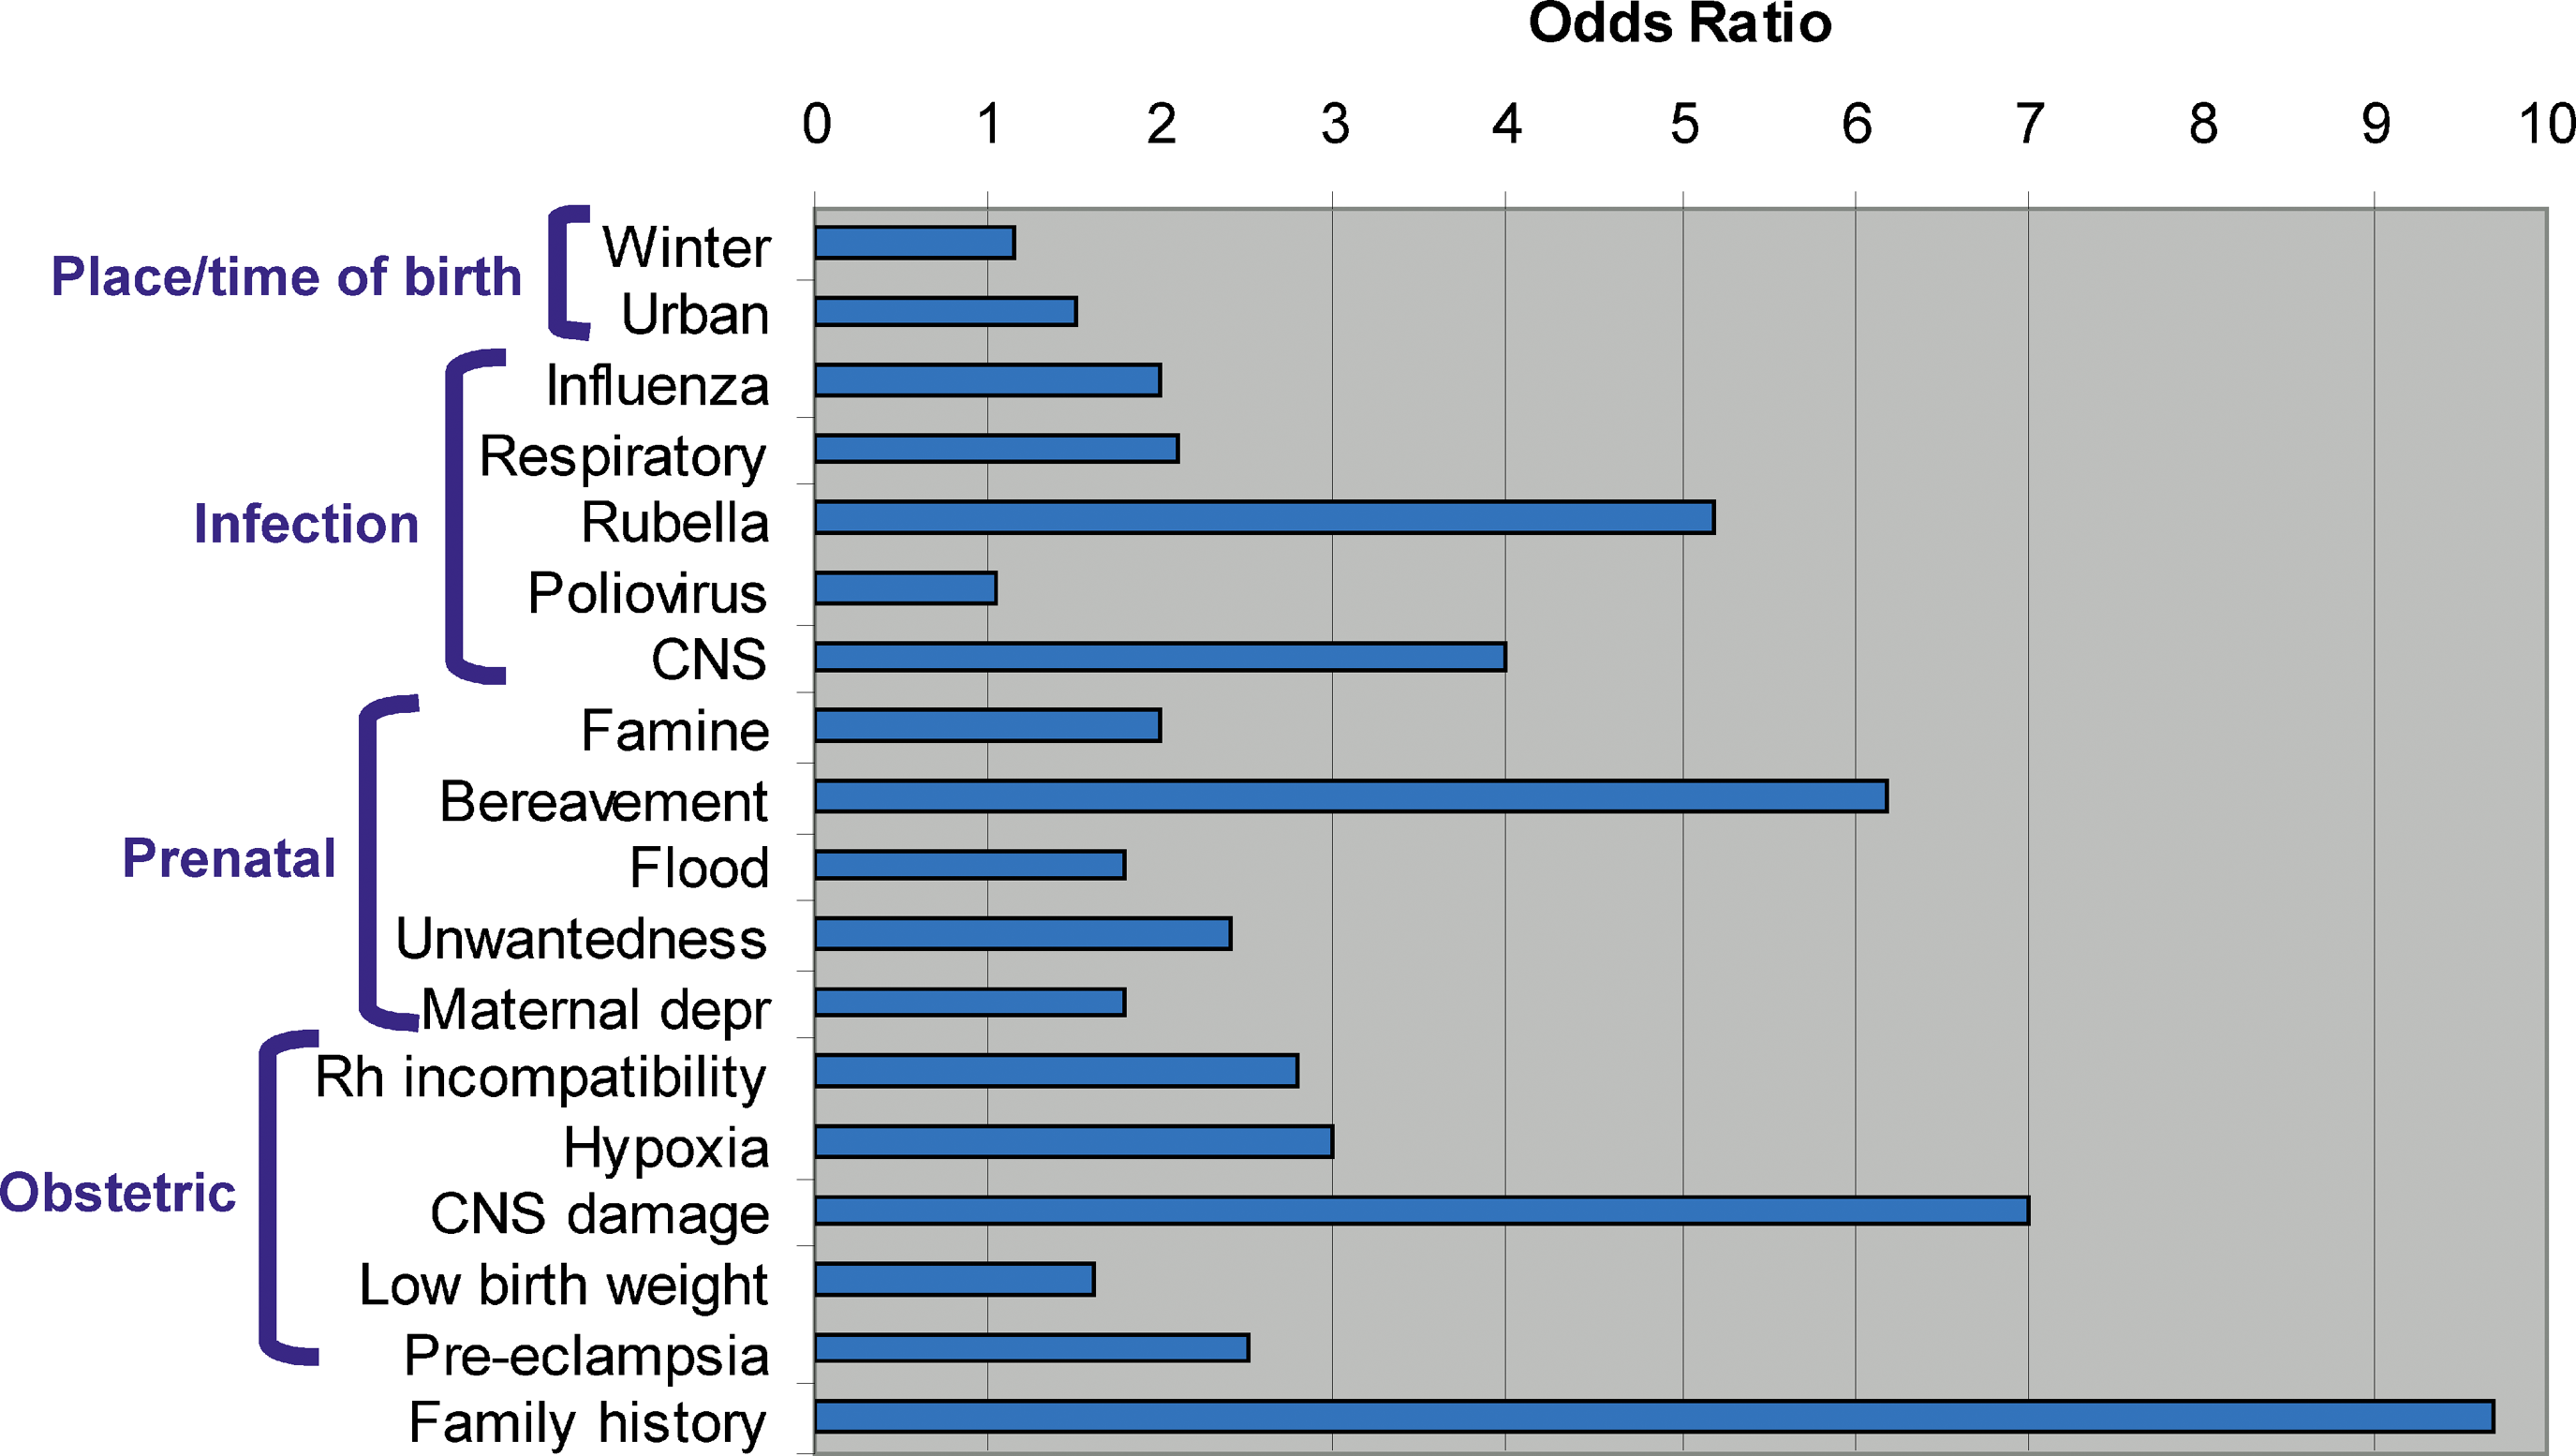
\includegraphics[width=\textwidth]{figure/risk_factors_of_schizophrenia.png}
		\caption[Risk factors of \glng{scz}]{Risk factors of \glng{scz}.
			It was observed that family history of \glng{scz} was the largest risk factors.
			Risk of \glng{scz} can be more than 9 times higher than the general population for individual with a family history of \glng{scz}}
		\label{fig:riskfactors}
	\end{figure}
	Prenatal infection has always been an important risk factor of \glng{scz}, being the single largest non-genetic risk factor of \glng{scz} (\cref{fig:riskfactors})\citep{Sullivan2005}.
	Initial clues indicated that births during the winter and spring months and in urban areas were related to an increased risk of the disorder \citep{Brown2010}.
	It was also observed that there was an increased risk of \glng{scz} in individuals who were fetuses during the 1957 influenza epidemic \citep{Mednick1958}.
	As the chance of getting infectious disease varies by season and infectious disease can spread more quickly in urban regions due to higher population density, these evidence suggest that prenatal infection might be associated with \glng{scz}.
	
	Early studies of prenatal infection in \glng{scz} mainly relies on ecological data such as influenza epidemics in the population to define the exposure status \citep{Brown2010}.
	The problem of these studies was that the exposure status was based solely on whether an individual was in gestation at the time of the epidemic without any confirmation of maternal infection during pregnancy.
	This leads to difficulties in replication of the findings.
	Subsequently, researchers uses birth cohorts where infection was documented using different biomarkers during pregnancies to provide a better labeling of the exposure status \citep{Brown2010}.
	Through these rigorous studies it was found that the risk of \glng{scz} increases as long as an individual's mother was infected by different form of infectious agents such as influenza, HSV-2 and \textit{T.gondii} during gestation \citep{Brown2010}.
	As different infectious agents all increase the risk of \glng{scz}, it leads to the hypothesis of \gls{mia} \citep{Brown2010} where it was suggested that instead of a particular infectious agents, it was the maternal immune response that disrupt the brain development in the offspring, thus leading to an elevated risk of \glng{scz}.
	
	To really understand how \gls{mia} increase the risk of \glng{scz}, it is important to understand the molecular mechanism.
	A great challenge in the study of \gls{mia} was that one cannot carry out empirical experiment in human samples due to ethical concerns.
	Thus a popular alternative is to employ rodent models.
	However, unlike physiological traits, psychiatric disorder such as that of \glng{scz} often contain symptoms related to higher level functioning such as hallucinations, delusion, disorganized speech etc \citep{AmericanPsychiatricAssociation2013} that are not readily detectable in rodents.
	This raises challenge in diagnosing whether if the rodent has demonstrated the symptoms of \glng{scz} for not only it was difficult to check whether if the high level functioning of the rodent is disrupted, there were no available biomarkers for \glng{scz}.
	Therefore instead of labeling whether if the rodent is ``schizophrenic'' or ``normal'', one would rather consider whether if the rodent demonstrate any ``schizophrenia-like'' behaviours such as impaired prepulse inhibition, impaired working memory and reduced social interaction \citep{Meyer2007a}.
	An important point to note here is that as autism and \glng{scz} shares most of these behavioral abnormality, and that risk of autism is also increased by \gls{mia} \citep{Brown2012}, studies using these rodent models were usually non-specific to \glng{scz} or autism. 
	Rather, autism and \glng{scz} were usually considered together in these models.
	However, the discussion of the etiology of autism and the similarity and difference between autism and \glng{szc} is beyond the scope of the current thesis.
	Therefore, for the simplicity and focus of the current thesis, we would limit our discussion to \glng{scz}.
	
	A common rodent model in the study of effect of \gls{mia} is to use the viral analogue \gls{polyic} to induce the maternal immune response during pregnancy in rodents.
	It was found that offspring exposed to \gls{polyic} displays phenotypes mirrors that observed in schizophrenia \citep{Li2009c,Meyer2009b,Li2010a} such as deficiency in prepulse inhibition \citep{Cadenhead2000}.
	Because \gls{polyic} only induce the \gls{mia} without infecting the fetuses, the \gls{polyic} model provide strong evidence that \gls{mia}, instead of the specific infection, contributes to the increased risk of \glng{scz}.	
	
	\citet{Smith2007} were able to demonstrate that a single injection of \gls{il6} to the pregnant mouse can induce \glng{scz}-like behaviour in the adult offspring. 
	What was most interesting was by eliminating the \gls{il6} from the maternal immune response using either genetic methods (\gls{il6} knock out) or with blocking antibodies, the behaviour deficits associated with \gls{mia} were not present in the adult offspring, suggesting that \gls{il6} is central to the process by which \gls{mia} causes long-term behavioral changes.
	
	Further studies of global gene expression patterns in \gls{mia}-exposed rodent fetal brains \citep{Oskvig2012,Garbett2012a} suggest that the post-pubertal onset of schizophrenic and other psychosis-related phenotypes might stem from attempts of the brain to counteract the environmental stress induced by \gls{mia} during its early development \citep{Garbett2012a}.
	For example, genes with neuroprotective function such as crystallins might also have additional roles in neuronal differentiation and axonal growth \citep{Garbett2012a}. 
	By over-expressing these genes to counteract the environmental stress, the balance between neurogenesis and differentiation in the embryonic brain maybe disrupted. 
	Based on these observations, \citet{Garbett2012a} propose that once the immune activation disappears, the normal brain development programme resumes with a time lag, result in permanent changes in connectivity and neurochemistry that might ultimately leads to \glng{scz}-like behaviours.
	\begin{figure}
		\centering
		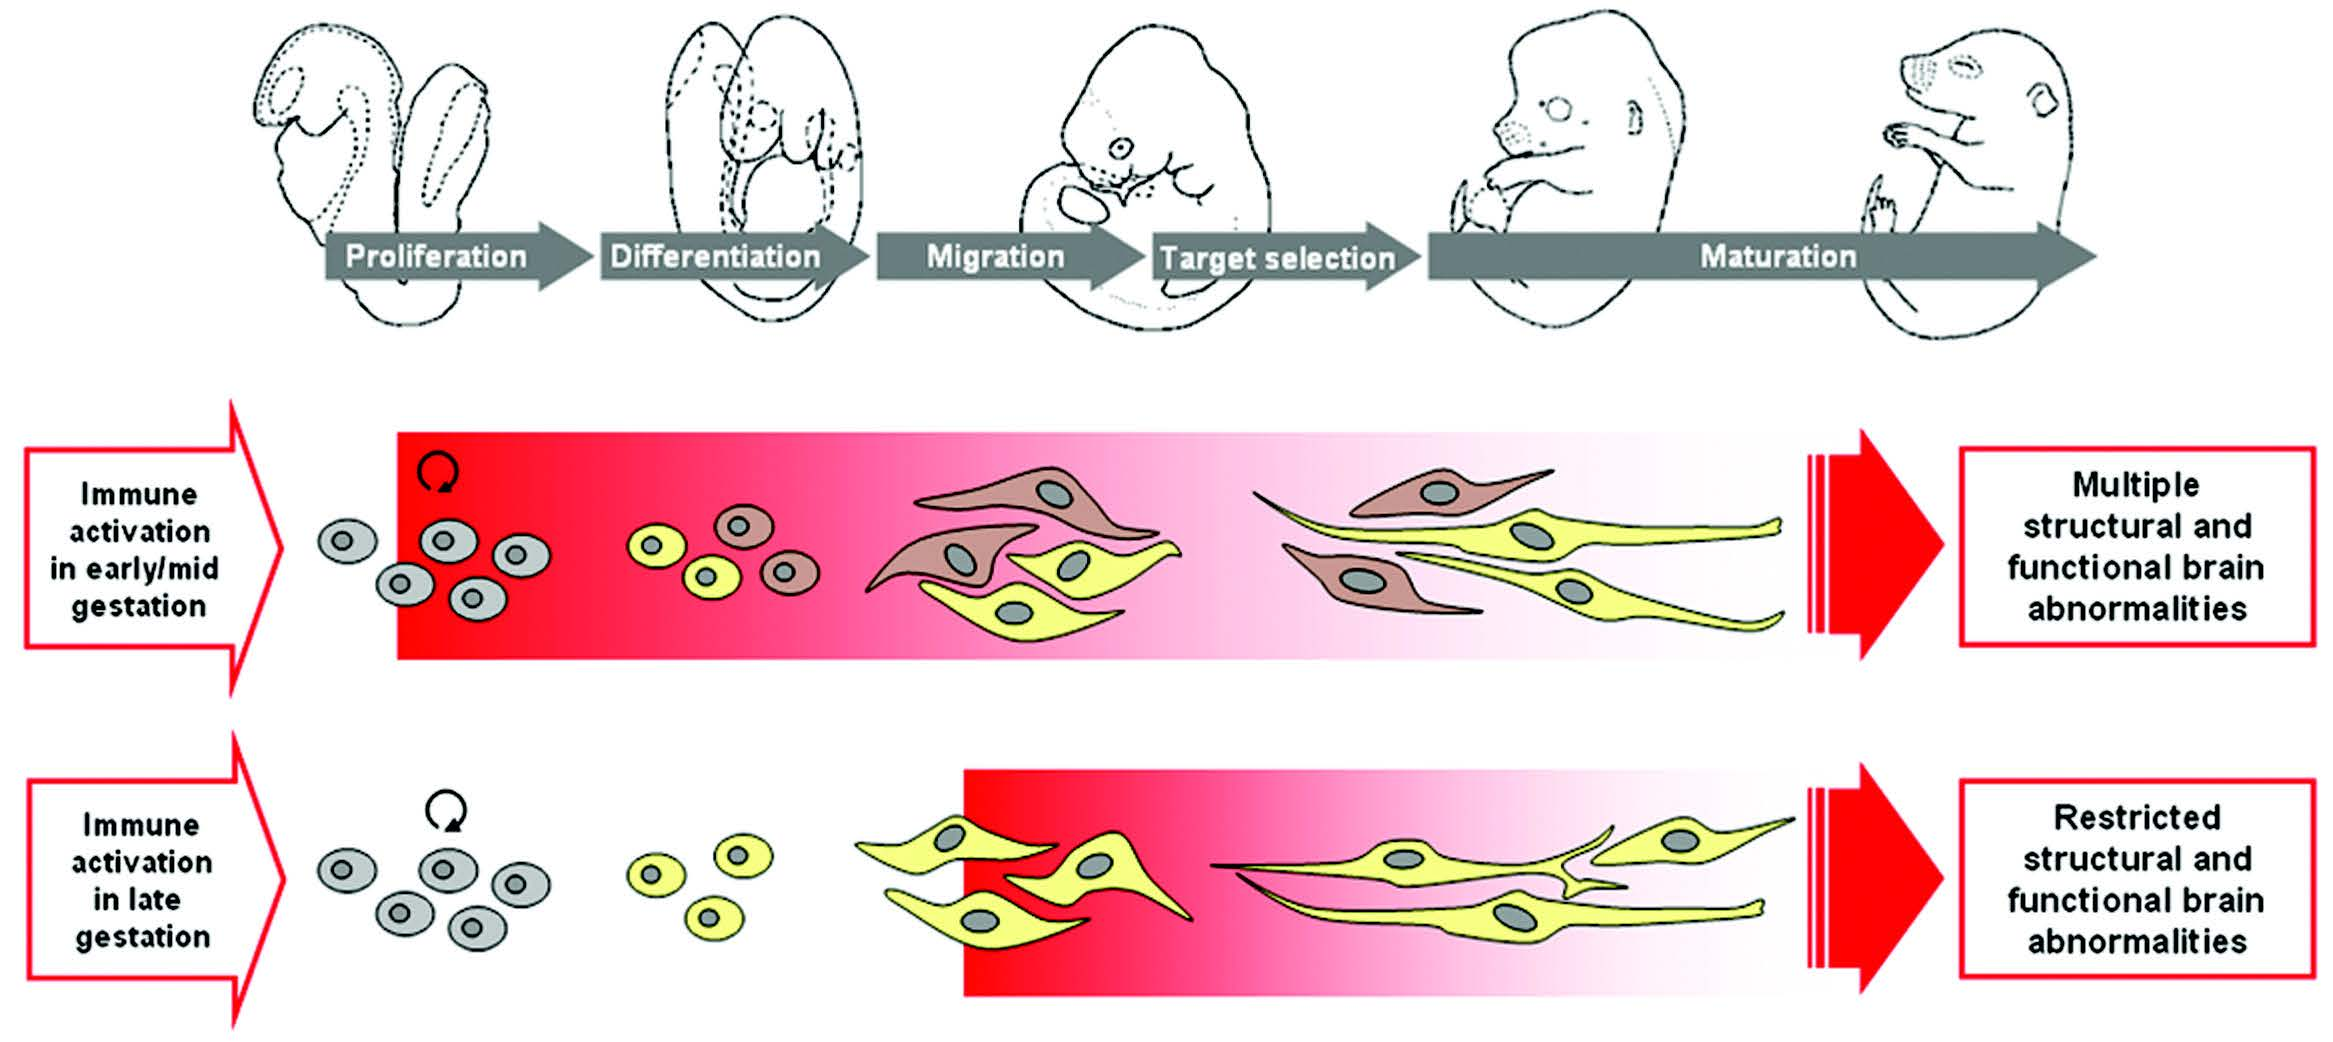
\includegraphics[width=\textwidth]{figure/mia_impact.jpg}
		\caption[Hypothesized model of the impact of prenatal immune challenge on fetal brain development]{Hypothesized model of the impact of prenatal immune challenge on fetal brain development.
			Maternal infection in early/mid pregnancy may affect early neurodevelopmental events in the fetal brain, thereby influencing the differentiation of neural precursor cells (grey) into particular neuronal phenotype (yellow or brown).
			This may predispose the developing fetal nervous system to additional failures leading to multiple structural and functional brain abnormalities in later life.
			Figure used with permission from Journal \citep{Meyer2007a}}
		\label{fig:miaEffect}
	\end{figure}
	
	On the other hand, an age dependent structural abnormalities in the mesoaccumbal and nigrostriatal dopamine systems were also found to be induced by \gls{mia} \citep{Vuillermot2010}.
	Specifically, \gls{mia} induces an early abnormality in specific dopaminergic systems such as those in the striatum and midbrian region \citep{Vuillermot2010}.
	Based on these observations, \citet{Meyer2007a} hypothesize that inflammation in the fetal brain during early gestation not only can disrupt neurodavelopmental processes such as cell proliferation and differentiation, it also predispose the developing nervous system to additional failures in subsequent cell migration, target selection, and synapse maturation (\cref{fig:miaEffect}) \citep{Meyer2007a}.
		
	In a separate study by \citet{Giovanoli2013}, mice were exposed to a lower dosage of \gls{polyic} during early gestation.
	Offspring born were then left undisturbed or exposed to unpredictable stress during peripubertal development.
	It was observed that offspring exposed to \gls{polyic} has an increased level of dopamine in the nucleus accumbens independent to whether if they were exposed to postnatal stress whereas serotonin (5-HT) were decreased in the medial prefrontal cortex when exposed to postnatal stress regardless of prenatal exposure.
	Only when the offspring were exposed to both \gls{polyic} and postnatal stress will they have an increased dopamine levels in the hippocampus or will sensorimotor gating and psychotomimetic drug sensitivity be affected \citep{Giovanoli2013}.
	\citet{Giovanoli2013} therefore suggest that the prenatal insult serves as a ``disease primer'' that increase offspring's vulnerability to subsequent insults.
	
	Together, these results supports the involvement of \gls{mia} in the development of \glng{scz}.
	It was even estimated that one third of all \glng{scz} cases could have been prevented shall all infection were prevented from the entire pregnant population \citep{Brown2010}.
	
	One of the critical consideration in the study of \gls{mia} is the specific gestation period of vulnerability to infection-mediated disturbance \citep{Meyer2007a}.
	Early epidemiological studies have suggested that the second trimester of human pregnancy might have been the vulnerability period.
	However, in the birth cohorts such as the Prenatal Determinants of \Gls{scz}, it was found that the time window with maximal risk for infection-mediated disturbance in brain development is earlier than the second trimester of human pregnancy and can be as early as the first trimester \citep{Meyer2007a}.
	Through the review of existing \gls{mia} studies on rodent models, \citet{Meyer2007a} suggests that effect of \gls{mia} during late pregnancy can be restricted to the late developmental programmes, thus have a more restricted pathological phenotype in the grown offspring compared to \gls{mia} during early pregnancy \citep{Meyer2007a}.
	Subsequent \gls{mia} studies using the \gls{polyic} mouse model also support the hypothesis proposed by \citet{Meyer2007a}, where it was observed that \gls{mia} early in gestation event might exert a more extensive impact on the phenotype of offspring \citep{Li2009c,Li2010a}.

	Despite the more severe impact of \gls{mia} during early gestation, most \gls{mia} studies have been focusing on the mid-gestation period and the understanding of the full molecular implication of early \gls{mia} events in adult brain were lacking.
	As technology advances, we can now employ the RNA Sequencing technique to examine the global mRNA expression changes in the brain of the adult offspring exposed to \gls{mia} during early gestation.
	
	\subsection{RNA Sequencing}
	Before the development of the \gls{ngs}, one can only inspect the global expression changes using the microarray using probe hybridization.
	As \gls{ngs} developed, one can now use poly-T probes to ``extract'' the mRNA fragments and sequence them.
	The depth of coverage of each gene then provide a general representation of the concentration fo the mRNA in the cell.
	When compared to microarray, the RNA Sequencing has a number of advantages, most notably, because RNA Sequencing does not rely on specific probe hybridization, it doesn't suffer from bias introduced by probe performances such as signal saturation, cross-hybridization, background noises and non-specific hybridization \citep{Zhao2014}.
	Moreover, RNA Sequencing has the additional advantage that one can perform not only the differential expression analysis, but also detect alternative splicing events and de novo transcripts.
	
	However, the analysis of RNA Sequencing is more complicated when compared to microarray.
	The first hurdle in the analysis of RNA Sequencing data is the sequence alignment.
	RNA sequencing will typically generate sequence reads from the mRNA transcripts and only need to align these reads to either the genome or the transcriptome in order to be able to calculate the depth of coverage for each genes, thus allowing the differential expression analysis.
	The different alignment strategies have their own pros and cons.
	
	Alignment to transcriptomes were most straightforward as the reads were originated from the transcripts and should have sequence composition similar to the transcriptome. 
	The problem of transcriptome alignment is that multiple isoform can share the same exon, leading to read mapping uncertainties \citep{Li2011e}.
	Without taking into consideration of the uncertainties, the downstream analysis might be biased and inaccurate. 
	When one is only interested in analyzing the gene level expression difference, this complication might be unnecessary.
	
	On the other hand, alignment to the genome should help to reduce the problem of multiple mapping yet it will require a splice aware aligner such as TopHat2 \citep{Kim2013}, STAR \citep{Dobin2013} and MapSplice \citep{Wang2010}.
	The reason behind was that as the reads were originated from the mRNA where alternative splicing might have occurred, the reads might span multiple exons which were separated by intronic regions. 
	The splicing algorithm will be able to ``split'' the reads and correctly align them onto the exons. 
	with the accurate alignment, one can then quantify the ``expression'' of each individual genes.
	
	The expression of a gene is usually represented in terms of number of reads aligned to the gene. 
	Given this information, statistic analysis can then be performed on the count data. 
	Unlike microarray, where the signal usually follows a normal distribution \citep{Hoyle2002,Giles2003}, the distribution of the RNA Sequencing count data were more complicated.
	Early RNA Sequencing experiment assumes the gene expression counts follows the Poisson distribution \citep{Marioni2008} where the variance is assumed to be equal to the mean of the expression.
	However, it was found that the assumption of Poisson distribution is too restrictive where an over-dispersion was typically observed in RNA Sequencing data \citep{Anders2010}.
	Therefore, to overcome the problem of over-dispersion, modern RNA Sequencing statistical package usually models the RNA Sequencing counts using the negative binomial distribution \citep{Anders2010,Robinson2010} or the beta negative binomial distribution \citep{Trapnell2012} instead of the Poisson distribution.
	\begin{figure}
		\centering
		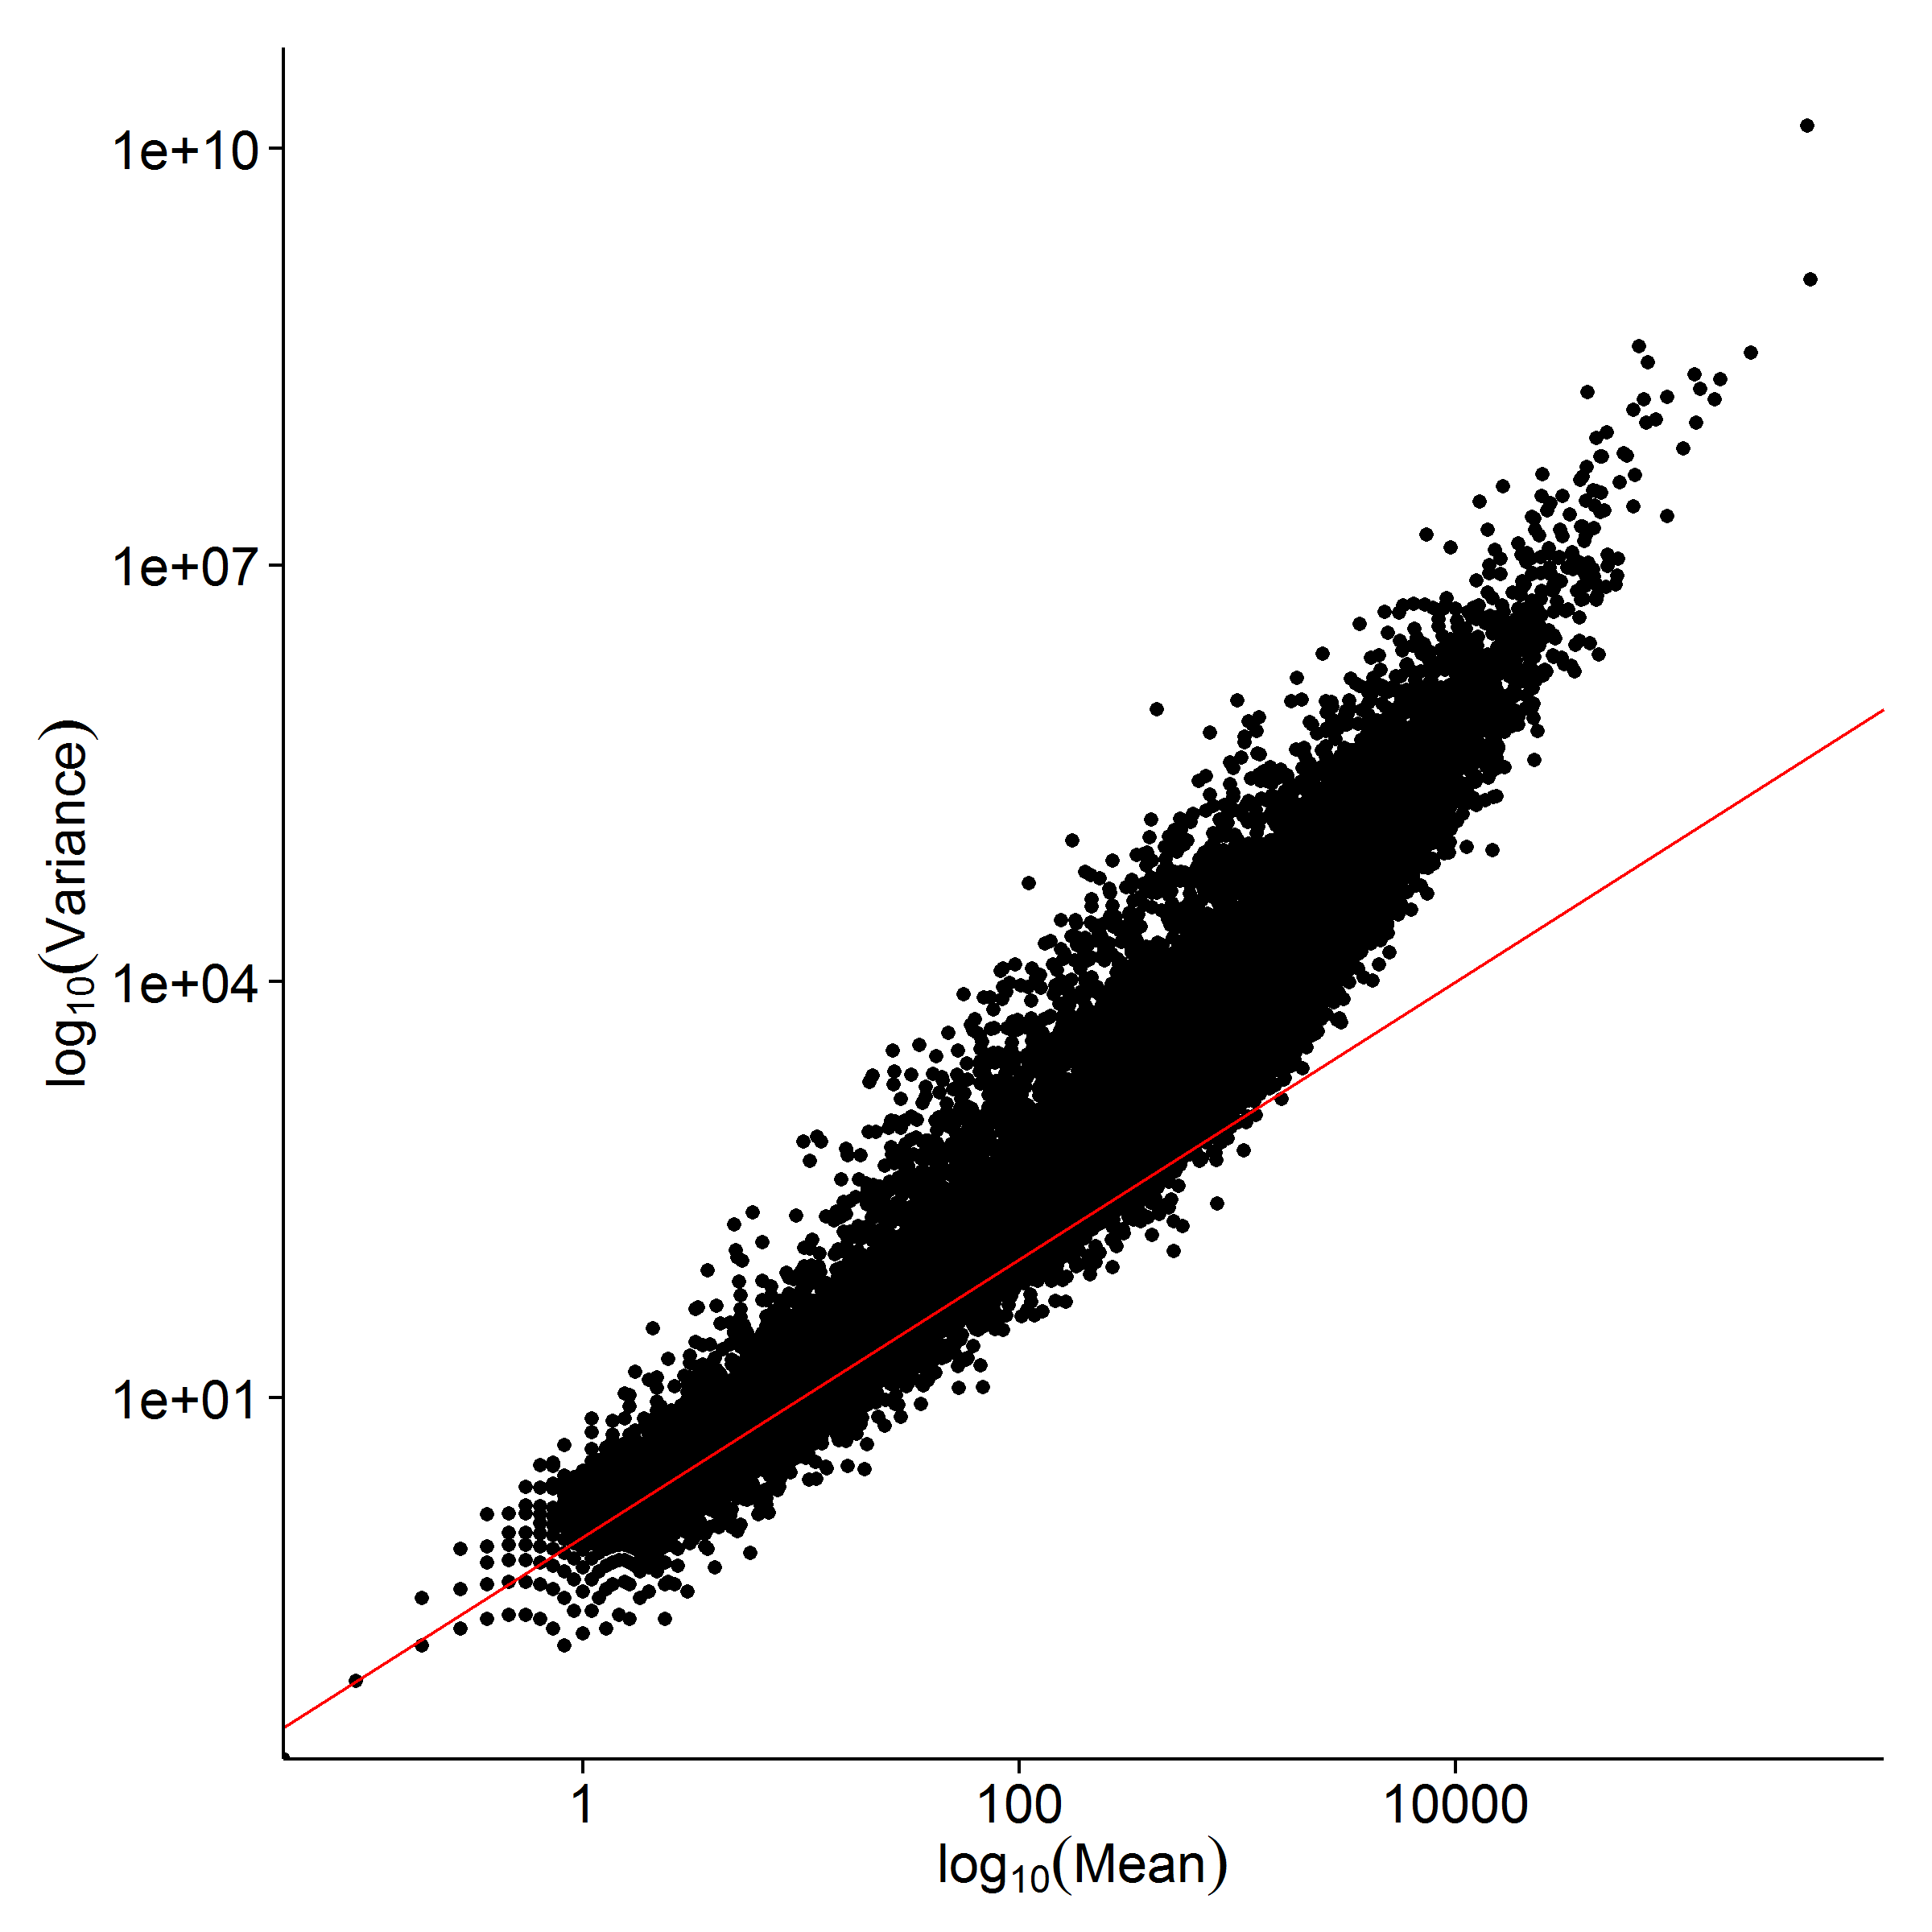
\includegraphics[width=0.5\textwidth]{figure/overdispersion.png}
		\caption[Over-dispersion observed in RNA Sequencing Count Data]{
			Over-dispersion observed in RNA Sequencing Count Data.
			If the RNA Sequencing count data follows the Poisson distribution, then the mean and variance of the data should be equal (follow the diagonal). 
			However, it was observed that as the mean increases, the variance increases even more, suggesting that there is an over-dispersion in the data. 
		}
	\end{figure}
	
	Nonetheless, as our knowledge with RNA Sequencing advances, we are getting better in utilizing the information provided by RNA Sequencing and it should serves as an important tool for the analysis of gene expression changes induced by \gls{mia} event.
	
	
	
	\section{Summary}
	In this thesis, we would like to first perform a series of empirical simulations to the effect of different genetic architectures and sampling strategies in \gls{GWAS} to the performance of \gls{ldsc}, for example, the effect of extreme phenotype samplings.
	On the other hand, as suggested by \citet{Bulik-Sullivan2015}, under certain conditions such as when the trait is oligogenic, the performance of \gls{ldsc} might be subpar. 
	Thus we would also like to develop an alternative algorithm for the estimation of \gls{SNP} heritability that is robust to different genetic architecture.
	Ultimately, we would like to repeat the analysis by \citet{Bulik-Sullivan2015} to estimate the true contribution of common \glspl{SNP} to the variance in \glng{scz}.

	Currently, there are evidences suggesting that there might be interaction between prenatal infection and genetic variations in the development of \glng{scz} \citep{Tienari2004,Clarke2009}.
	We therefore hypothesize that the differential gene expression induced by \gls{mia} and genetic mutation might have act upon the same functional pathway.
	To test this hypothesis, we performed a hypothesis generation RNA Sequencing study to capture gene expression changes induced by early \gls{mia} events (\gls{gd}9) in the cerebellum of mouse using the \gls{polyic} mouse model.
	Based on the gene expression changes, we hope to identify pathways perturbed by early \gls{mia} events.
	Most importantly, we would like to test whether if these pathways contribute disproportionately to the heritability of \glng{scz}.
	As a result of that, we would also perform the partitioning of heritability using \gls{ldsc} on the pathways affected by \gls{mia}.
	
	Moreover, recent study from our lab suggested that n-3 \gls{pufa} rich diet might help to reduce the \glng{scz}-like behaviour in mice exposed to early \gls{mia} insults \citep{Li2015}. 
	Therefore we would also like to take this opportunity to assess the effect of n-3 \gls{pufa} rich diet on the gene expression pattern in the brain of the adult offspring.
	
	This thesis will be divided into three parts.
	First, in \Cref{heritabilityChapter}, we performed a series of empirical simulations to assess the performance of \gls{ldsc} in the estimation of \gls{SNP} heritability. 
	We also proposed an alternative approach for the estimation of \gls{SNP}-heritability from \gls{GWAS} summary statistics that is robust to different genetic architectures.
	
	In \Cref{omegaProject}, a hypothesis generation study was performed to study the effect of \gls{mia} on the gene expression pattern of mouse cerebellum. 
	On top of that, as recent study suggested that n-3 \gls{pufa} rich diet can help to reduce the \glng{scz}-like behaviour observed mouse exposed to early \gls{mia} \citep{Li2015}, we also investigated the effect of n-3 \gls{pufa} rich diet on the gene expression pattern of mouse cerebellum.
	
	Lastly, we summarize and conclude all findings in \Cref{conclusionChapter} and give future perspectives on the \glng{szc} research.
	